\chapter{Resultados}
\label{cap_resultados}

Neste capítulo são exibidos os resultados obtidos da aplicação do algoritmo
desenvolvido na otimização de algumas funções. Na seção \ref{sec_test_functions}
o algoritmo é utilizado para acusar máximos de algumas funções de $\R^2$ em $\R$
e na seção \ref{sec_resultados_tmdcs} é feito o ajuste das bandas de energia
dos TMDCs \ch{CrS2} e \ch{CrSe2} minimizando o desvio quadrático médio entre
os autovalores da hamiltoniana do modelo $ k \cdot p $ e os respectivos níveis
calculados previamente via DFT. Por fim, com os parâmetros ajustados, são ilustrados
alguns resultados físicos relevantes.

\section{Testes em Funções}
\label{sec_test_functions}

Nessa seção são exibidos os resultados de alguns testes em funções reais em $\R^2$. Em cada teste, 
8 populações com 1000 indivíduos com cromossomos de 32 bits são evoluídas por 100 gerações. O espaço de busca
considerado foi $ [-1,1] \times [-1, 1] $, onde os indivíduos foram distribuídos aleatoriamente. 
O valor usado para o parâmetro da função desempenho foi $h = 2$,
as configurações para a elite foram $e_1 = 4$, $e_2 = 6$ e $e_3 = 10$ e as probabilidades de mutação $p_2$ e $p_3$ escolhidas
foram $p_2 = 5\%$ e $p_3 = 5\%$.

Ao final do processo,
foram gerados gráficos com as curvas de nível de cada função e com as posições de todos os
integrantes de todas as populações. Os 8 melhores indivíduos são marcados de forma distinta,
afim de atestar se o algoritmo foi capaz ou não de encontrar a solução real do problema.
Um segundo gráfico com os valores das funções dos 200 melhores indivíduos de cada população
no decorrer das gerações foi gerado, a fim de mostrar, em caso de convergência, sua rapidez.

Ambos os gráficos foram feitos novamente com probabilidades de mutação $p_2 = p_3 = 20\%$
para demonstrar o papel da mutação no decorrer do algoritmo, e averiguar seu impacto na diversidade genética
dos indivíduos.
Por fim, é feita uma breve discussão sobre a performance da implementação do algoritmo e sua
complexidade de tempo de execução.

A primeira função testada foi
\begin{align}
  \begin{split}    
    f_1(x,y) & = \cos(9\pi r)\exp\left\{-\frac{r^2}{(0,4)^2}\right\} \;\text{, com} \\
    r      & = \sqrt{
      \left(x - 0,5\right)^2 +
      \left(y - 0,5\right)^2
    }
  \end{split}
  \label{eq:func_damped_cossine}
\end{align}
cujo gráfico se encontra na Figura \ref{fig:graph_damped_cossine} e os
resultados obtidos estão dispostos nas Figuras \ref{fig:contour_damped_cossine},
\ref{fig:evolution_damped_cossine}, \ref{fig:contour_damped_cossine_mut_20} e 
\ref{fig:evolution_damped_cossine_mut_20}. A segunda função testada foi
\begin{align}
  \begin{split}
    f_2(x,y) & = 0,8 \exp\left\{-\frac{r_1^2}{(0,3)^2}\right\} +
    0,88 \exp\left\{-\frac{r_2^2}{(0,03)^2}\right\} \;\text{, onde} \\
    r_1      & = \sqrt{
      \left(x - 0,5\right)^2 +
      \left(y - 0,5\right)^2
    } \;\text{ e} \\
    r_2      & = \sqrt{
      \left(x - 0,6\right)^2 +
      \left(y - 0,1\right)^2
    } \mathcomma
  \end{split}
  \label{eq:func_near_gaussians}
\end{align}
cujo gráfico se encontra na Figura \ref{fig:graph_near_gaussians} com os
resultados obtidos ilustrados nas Figuras \ref{fig:contour_near_gaussians},
\ref{fig:evolution_near_gaussians}, \ref{fig:contour_near_gaussians_mut_20} e 
\ref{fig:evolution_near_gaussians_mut_20}.

Como pode ser observado, em todos os casos, os melhores indivíduos foram localizados 
com precisão no máximo global. Não obstante, uma variedade genética proporcional a
probabilidade de mutação foi mantida, dada uma escolha correta de $p_2$ e $p_3$ para cada
problema. Nos casos em que $p_2 = 20\%$, os indivíduos, ao final do processo, se encontravam
espalhados por todo o espaço de busca. 

Vale ressaltar porém que o valor necessário de $p_2$ e $p_3$ para que uma população 
tenha a distribuição desejada depende da função a ser otimizada, como pode ser visto
comparando as Figuras \ref{fig:contour_damped_cossine_mut_20} e \ref{fig:evolution_damped_cossine_mut_20}
com as Figuras \ref{fig:contour_near_gaussians_mut_20} e \ref{fig:evolution_near_gaussians_mut_20}.
Assim, a influência dos parâmetros $p_2$, $p_3$, $e_1$, $e_2$ e $e_3$ no comportamento da população
deve ser estudada em cada caso, afim de extrair do algoritmo o resultado desejado.

Outra vantagem do algoritmo é que os máximos locais também puderam ser encontrados.
Isso pode ser observado especialmente na Figura \ref{fig:evolution_damped_cossine_mut_20},
onde visivelmente há uma concentração de indivíduos em $ f_1(x,y) \approx 0,74 $ e 
$ f_1(x,y) \approx 0,29 $, que correspondem aos dois primeiros máximos locais.
Algo similar pode ser observado na segunda função, nas primeiras gerações da Figura 
\ref{fig:evolution_near_gaussians_mut_20}, com alguma concentração da população em
vermelho em $f_1(x,y) \approx 0,8$.

Claro que, mesmo nos casos em que não é possível inferir o máximo local da evolução
de uma parcela da população\trav como ocorre na Figura \ref{fig:evolution_damped_cossine}\trav
uma análise estatística feita sobre os valores das funções desempenho dos indivíduos e
suas respectivas posições ainda seria capaz de acusá-lo.

Em alguns casos, 100 gerações não são o suficiente para determinar a solução correta. Na população
em vermelho na Figura \ref{fig:evolution_near_gaussians} houve uma convergência rápida para o
máximo local, onde todos os 200 melhores indivíduos permaneceram durante toda a duração do teste.
Algo similar ocorreu na população em verde, para a maioria dos indivíduos da elite. Entretanto, 
o número de gerações sempre pode ser escolhido conforme a necessidade.

\begin{figure}
  \begin{subfigure}{\textwidth}
    \centering
    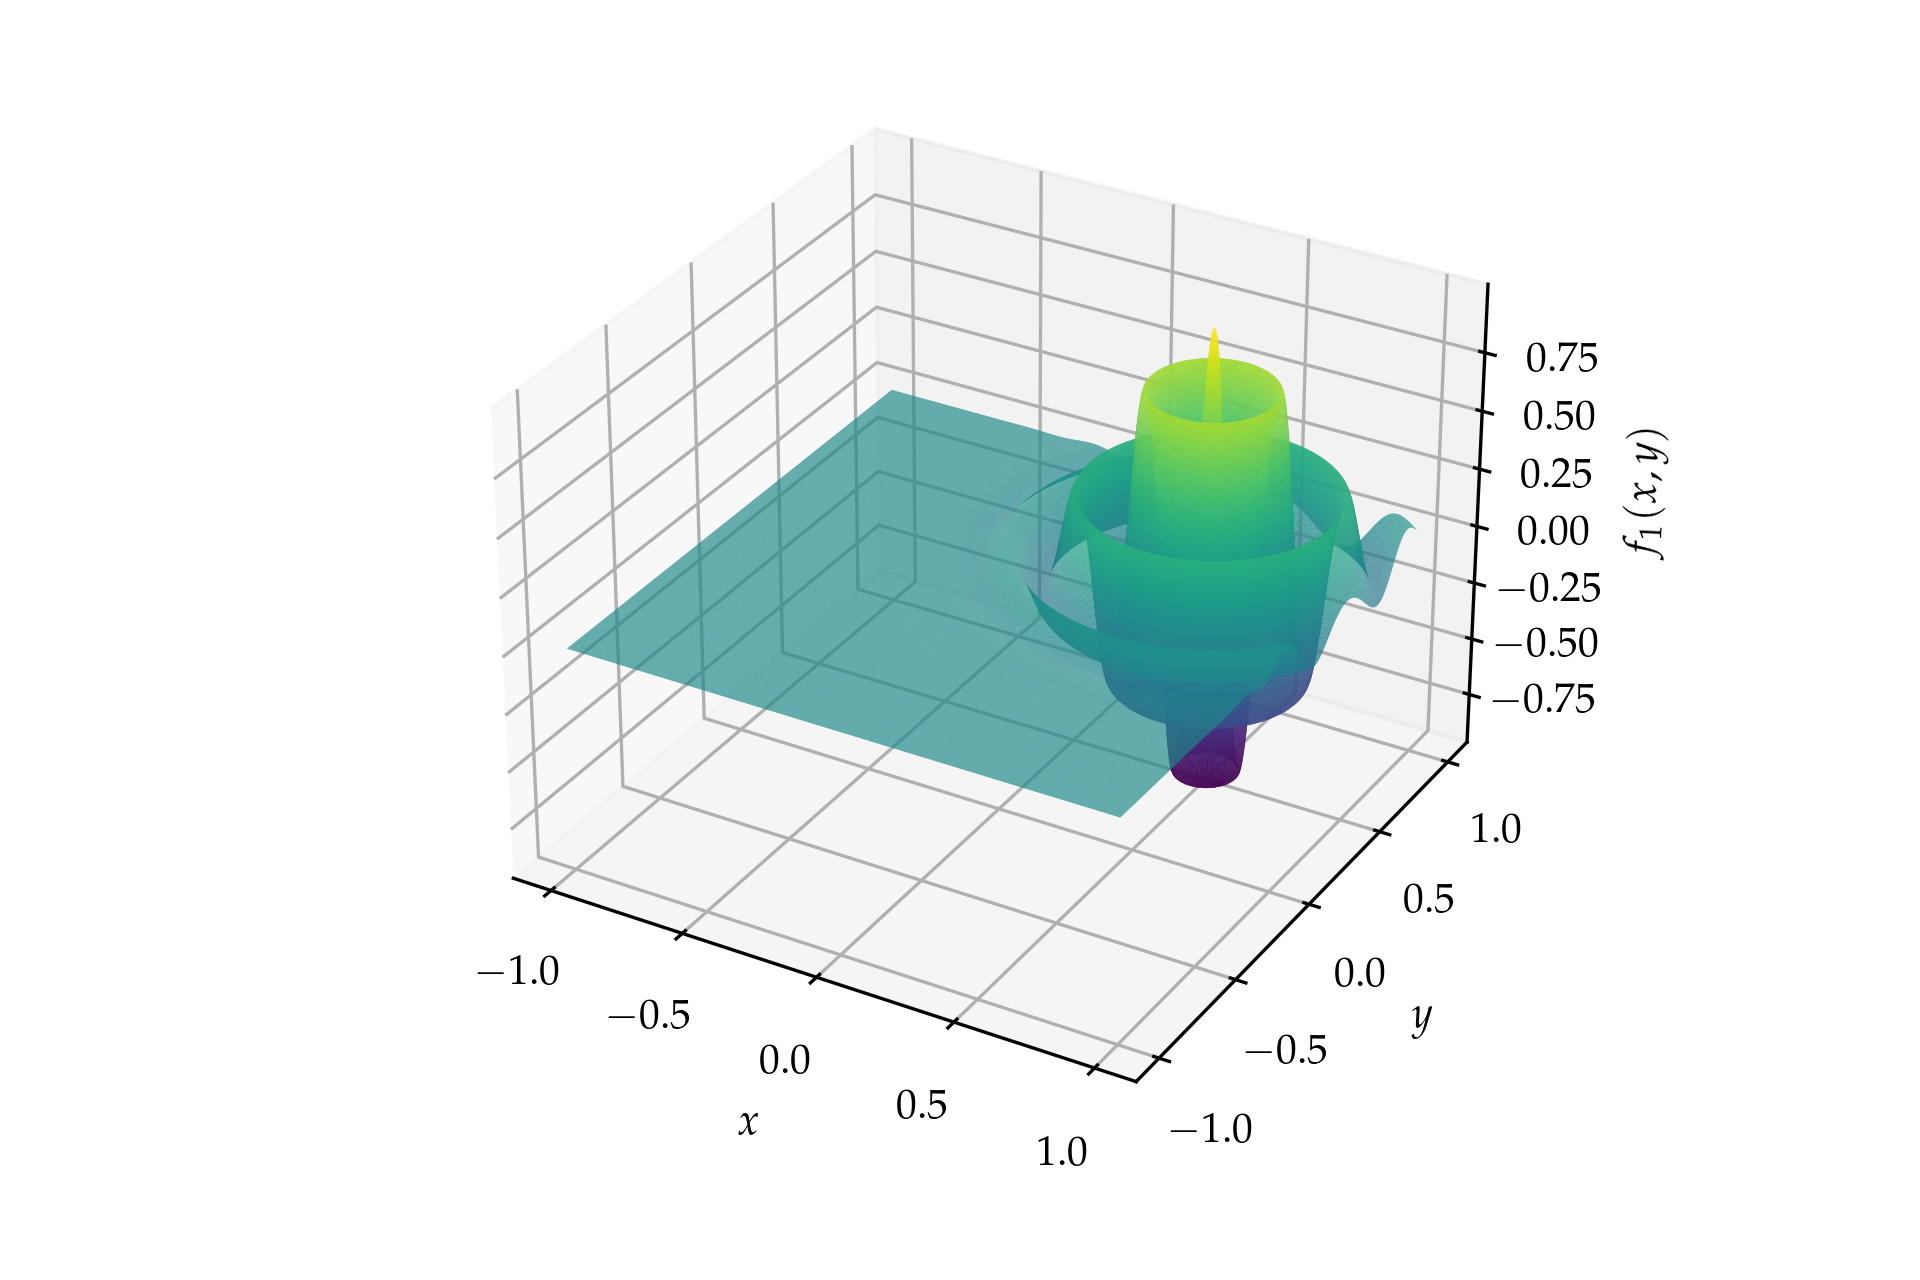
\includegraphics[width=\textwidth]{imagens/graph_damped_cossine.png}
    \caption{}
    \label{fig:graph_damped_cossine}
  \end{subfigure}
  \begin{subfigure}{\textwidth}
    \centering
    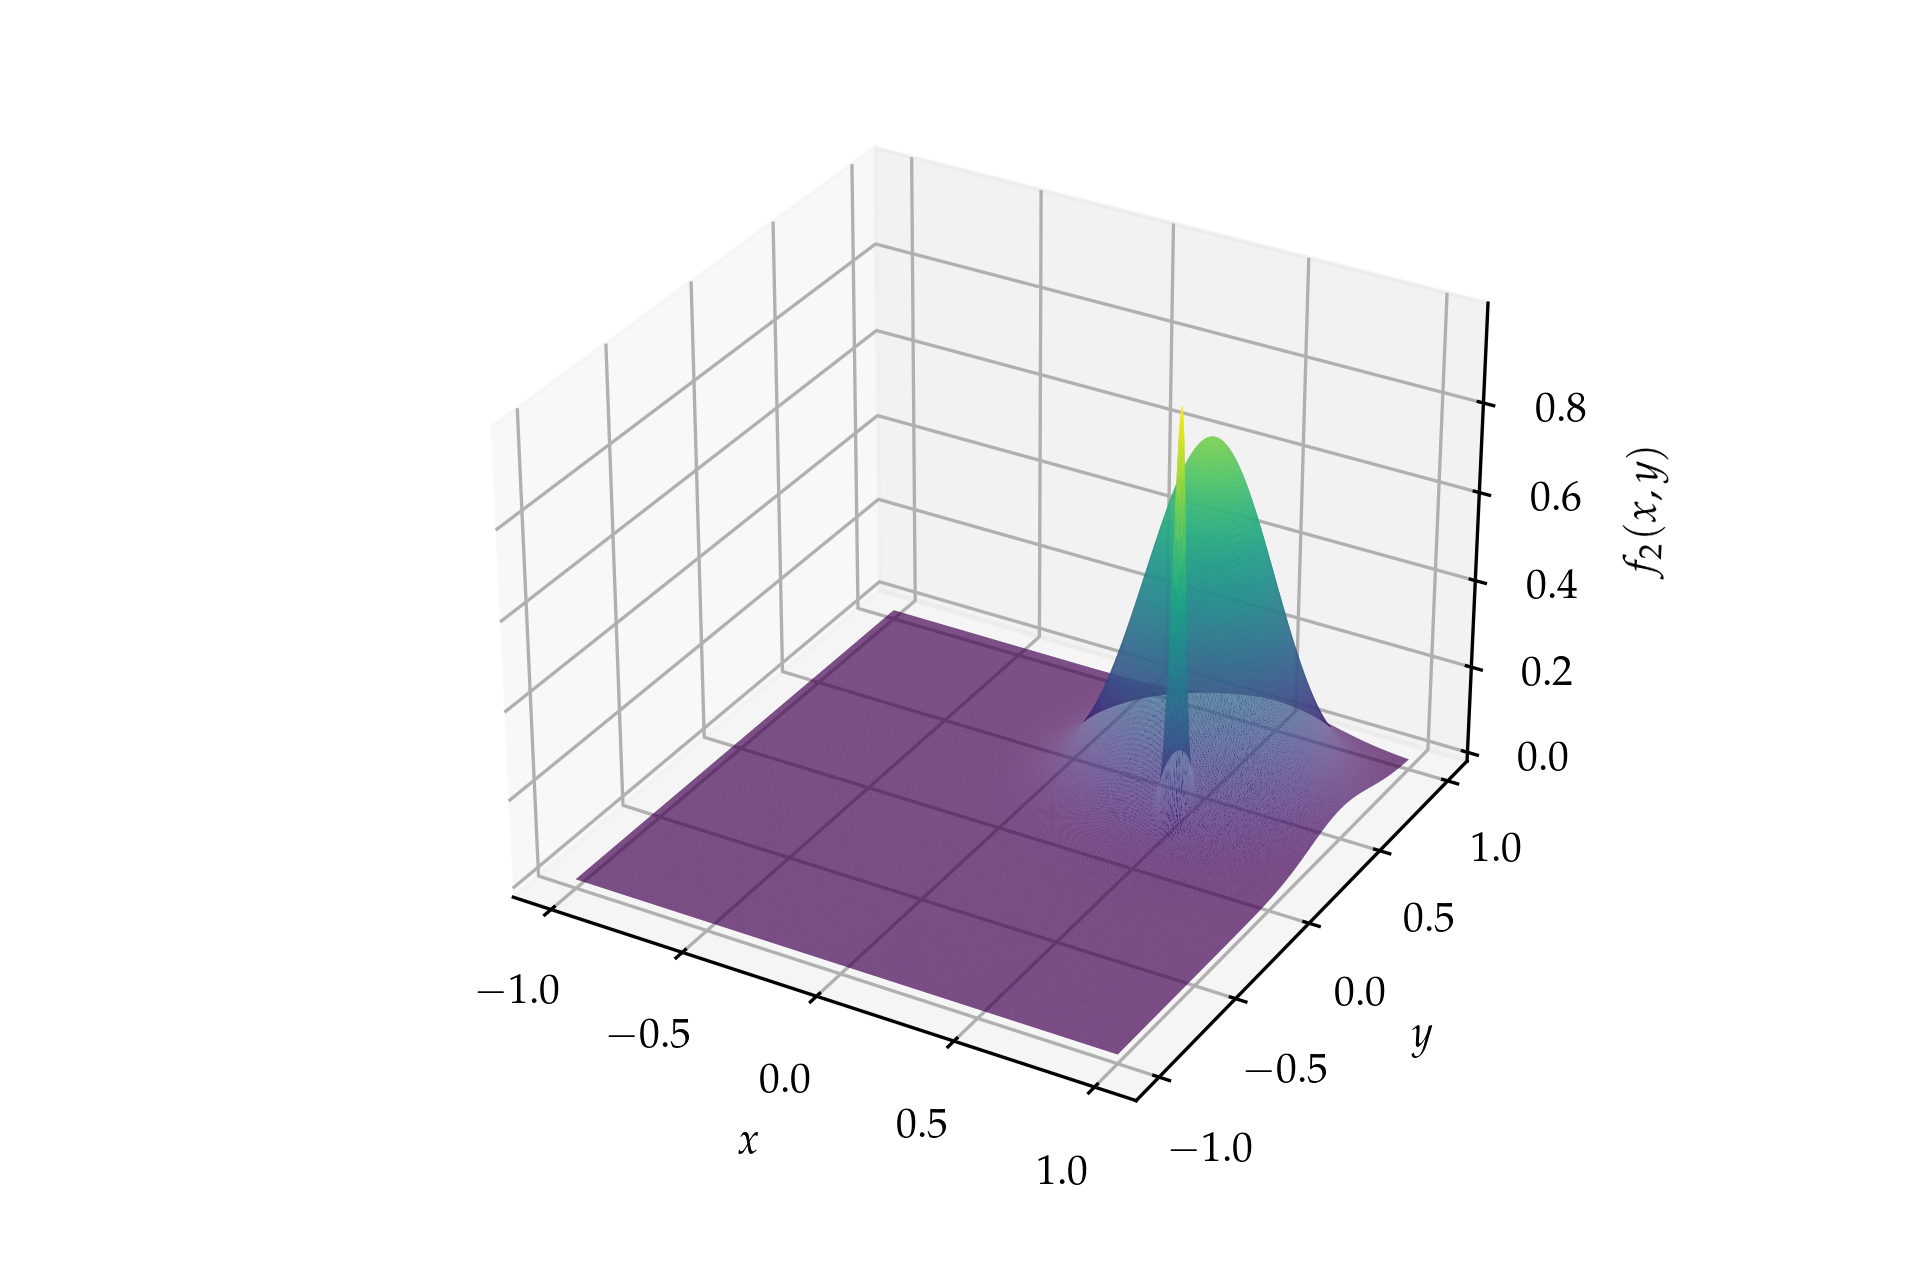
\includegraphics[width=\textwidth]{imagens/graph_near_gaussians.png}
    \caption{}
    \label{fig:graph_near_gaussians}
  \end{subfigure}
  \caption{
    \subref{fig:graph_damped_cossine} Gráfico da função $f_1(x,y)$.
    \subref{fig:graph_near_gaussians} Gráfico da função $f_2(x,y)$.
  }
\end{figure}

\begin{figure}[p]
  \centering
  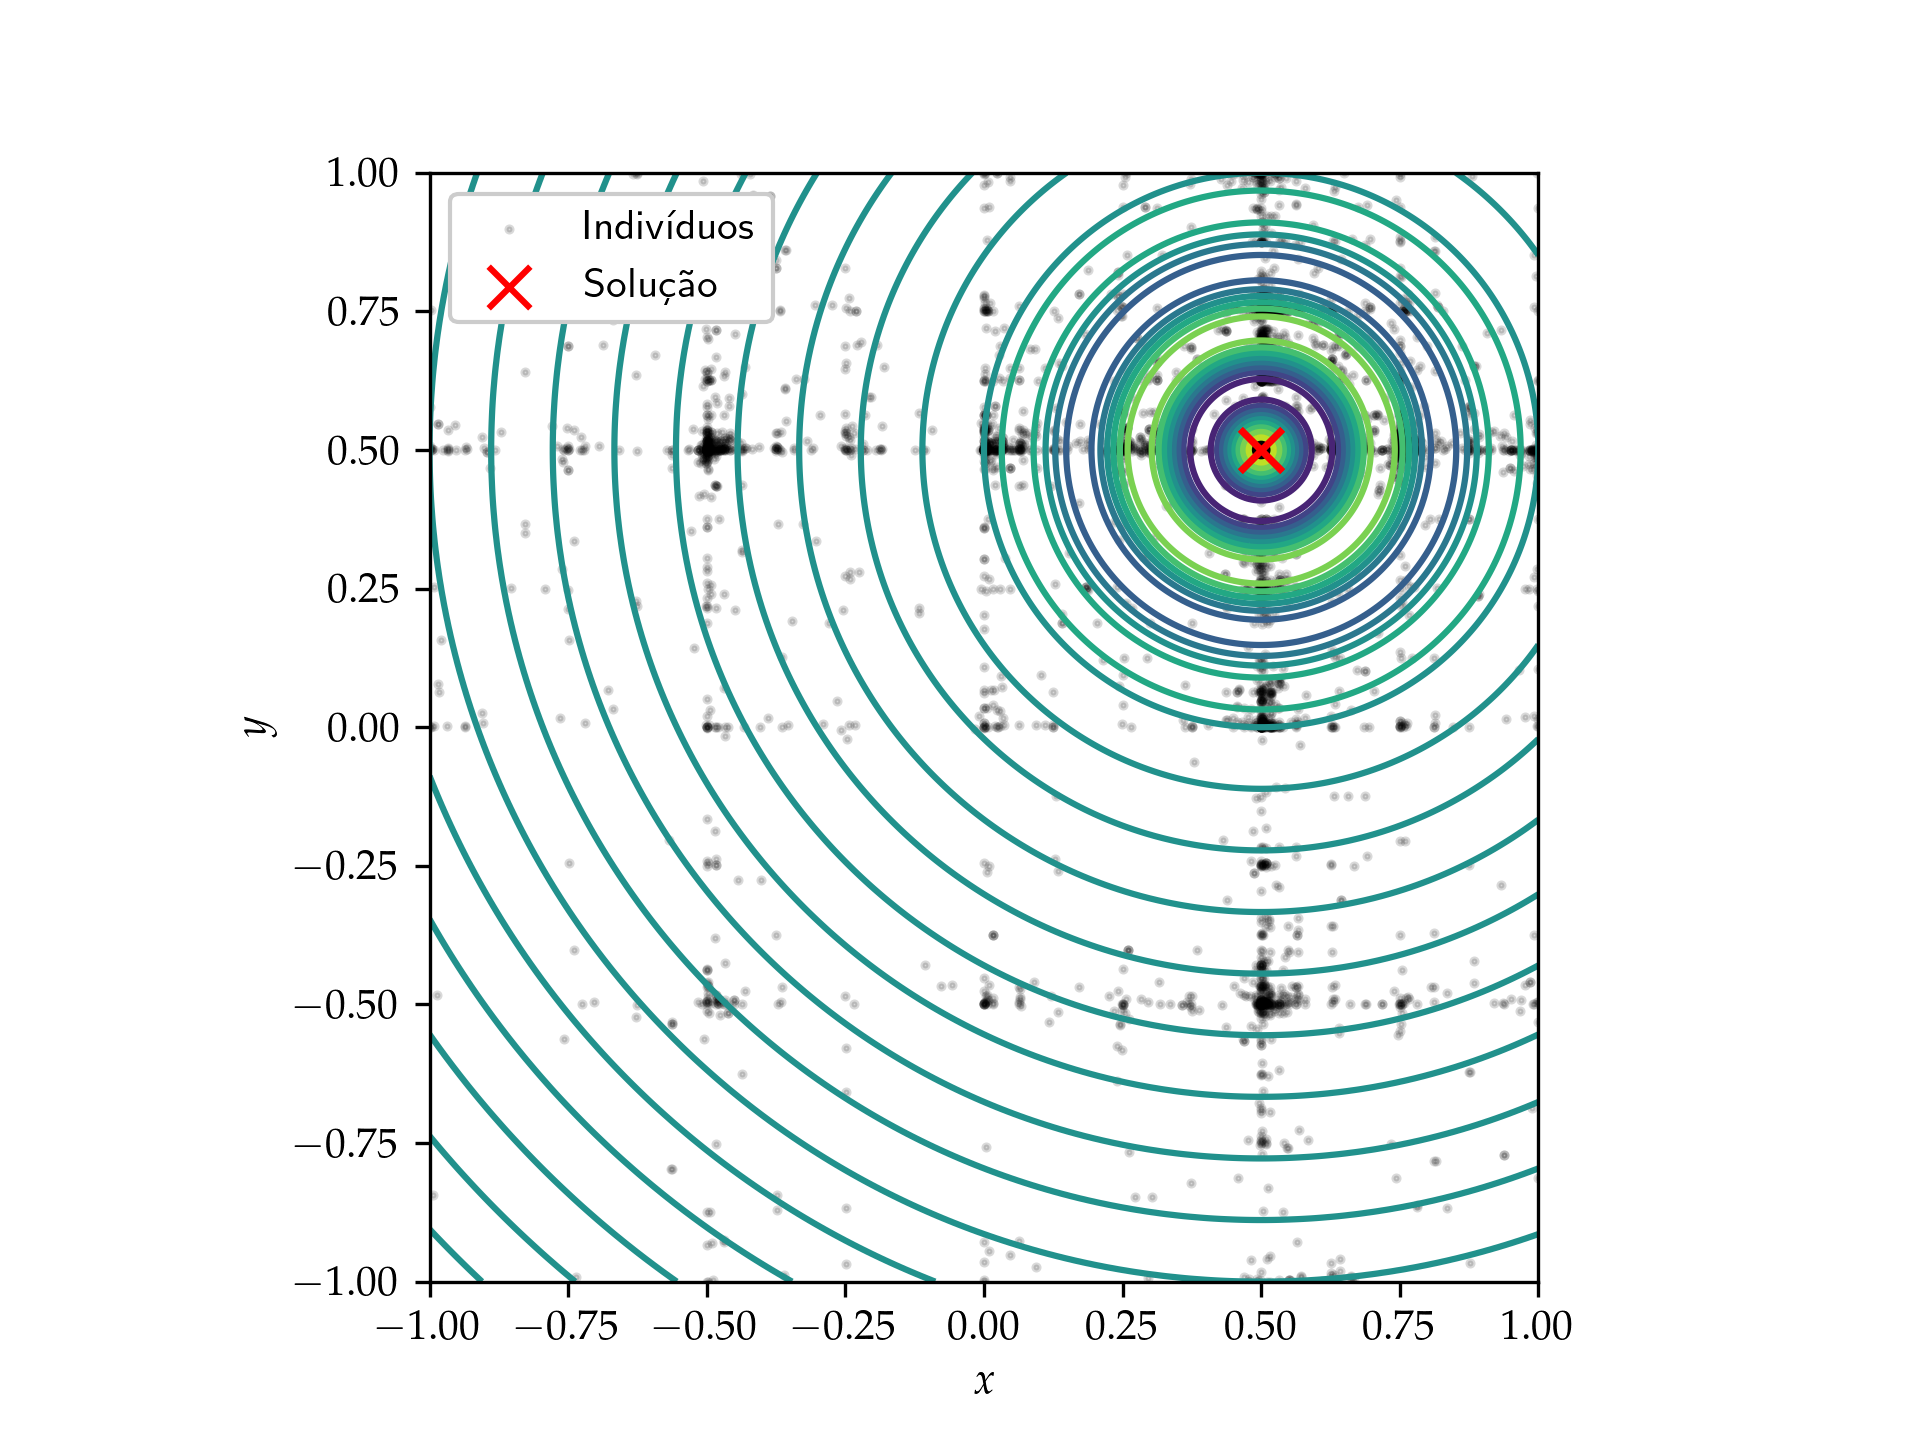
\includegraphics[width=\textwidth]{imagens/low_prob/contour_damped_cossine.png}
  \caption{
    Curvas de nível da função $f_1(x,y)$. Os pontos em preto indicam as posições dos indivíduos
    de 8 populações em sua 100ª geração na otimização da função, com $ p_2 = p_3 = 5\% $. 
    Marcado com um $\times$ vermelho estão os melhores indivíduos de cada população.
  }
  \label{fig:contour_damped_cossine}
\end{figure}

\begin{figure}[p]
  \centering
  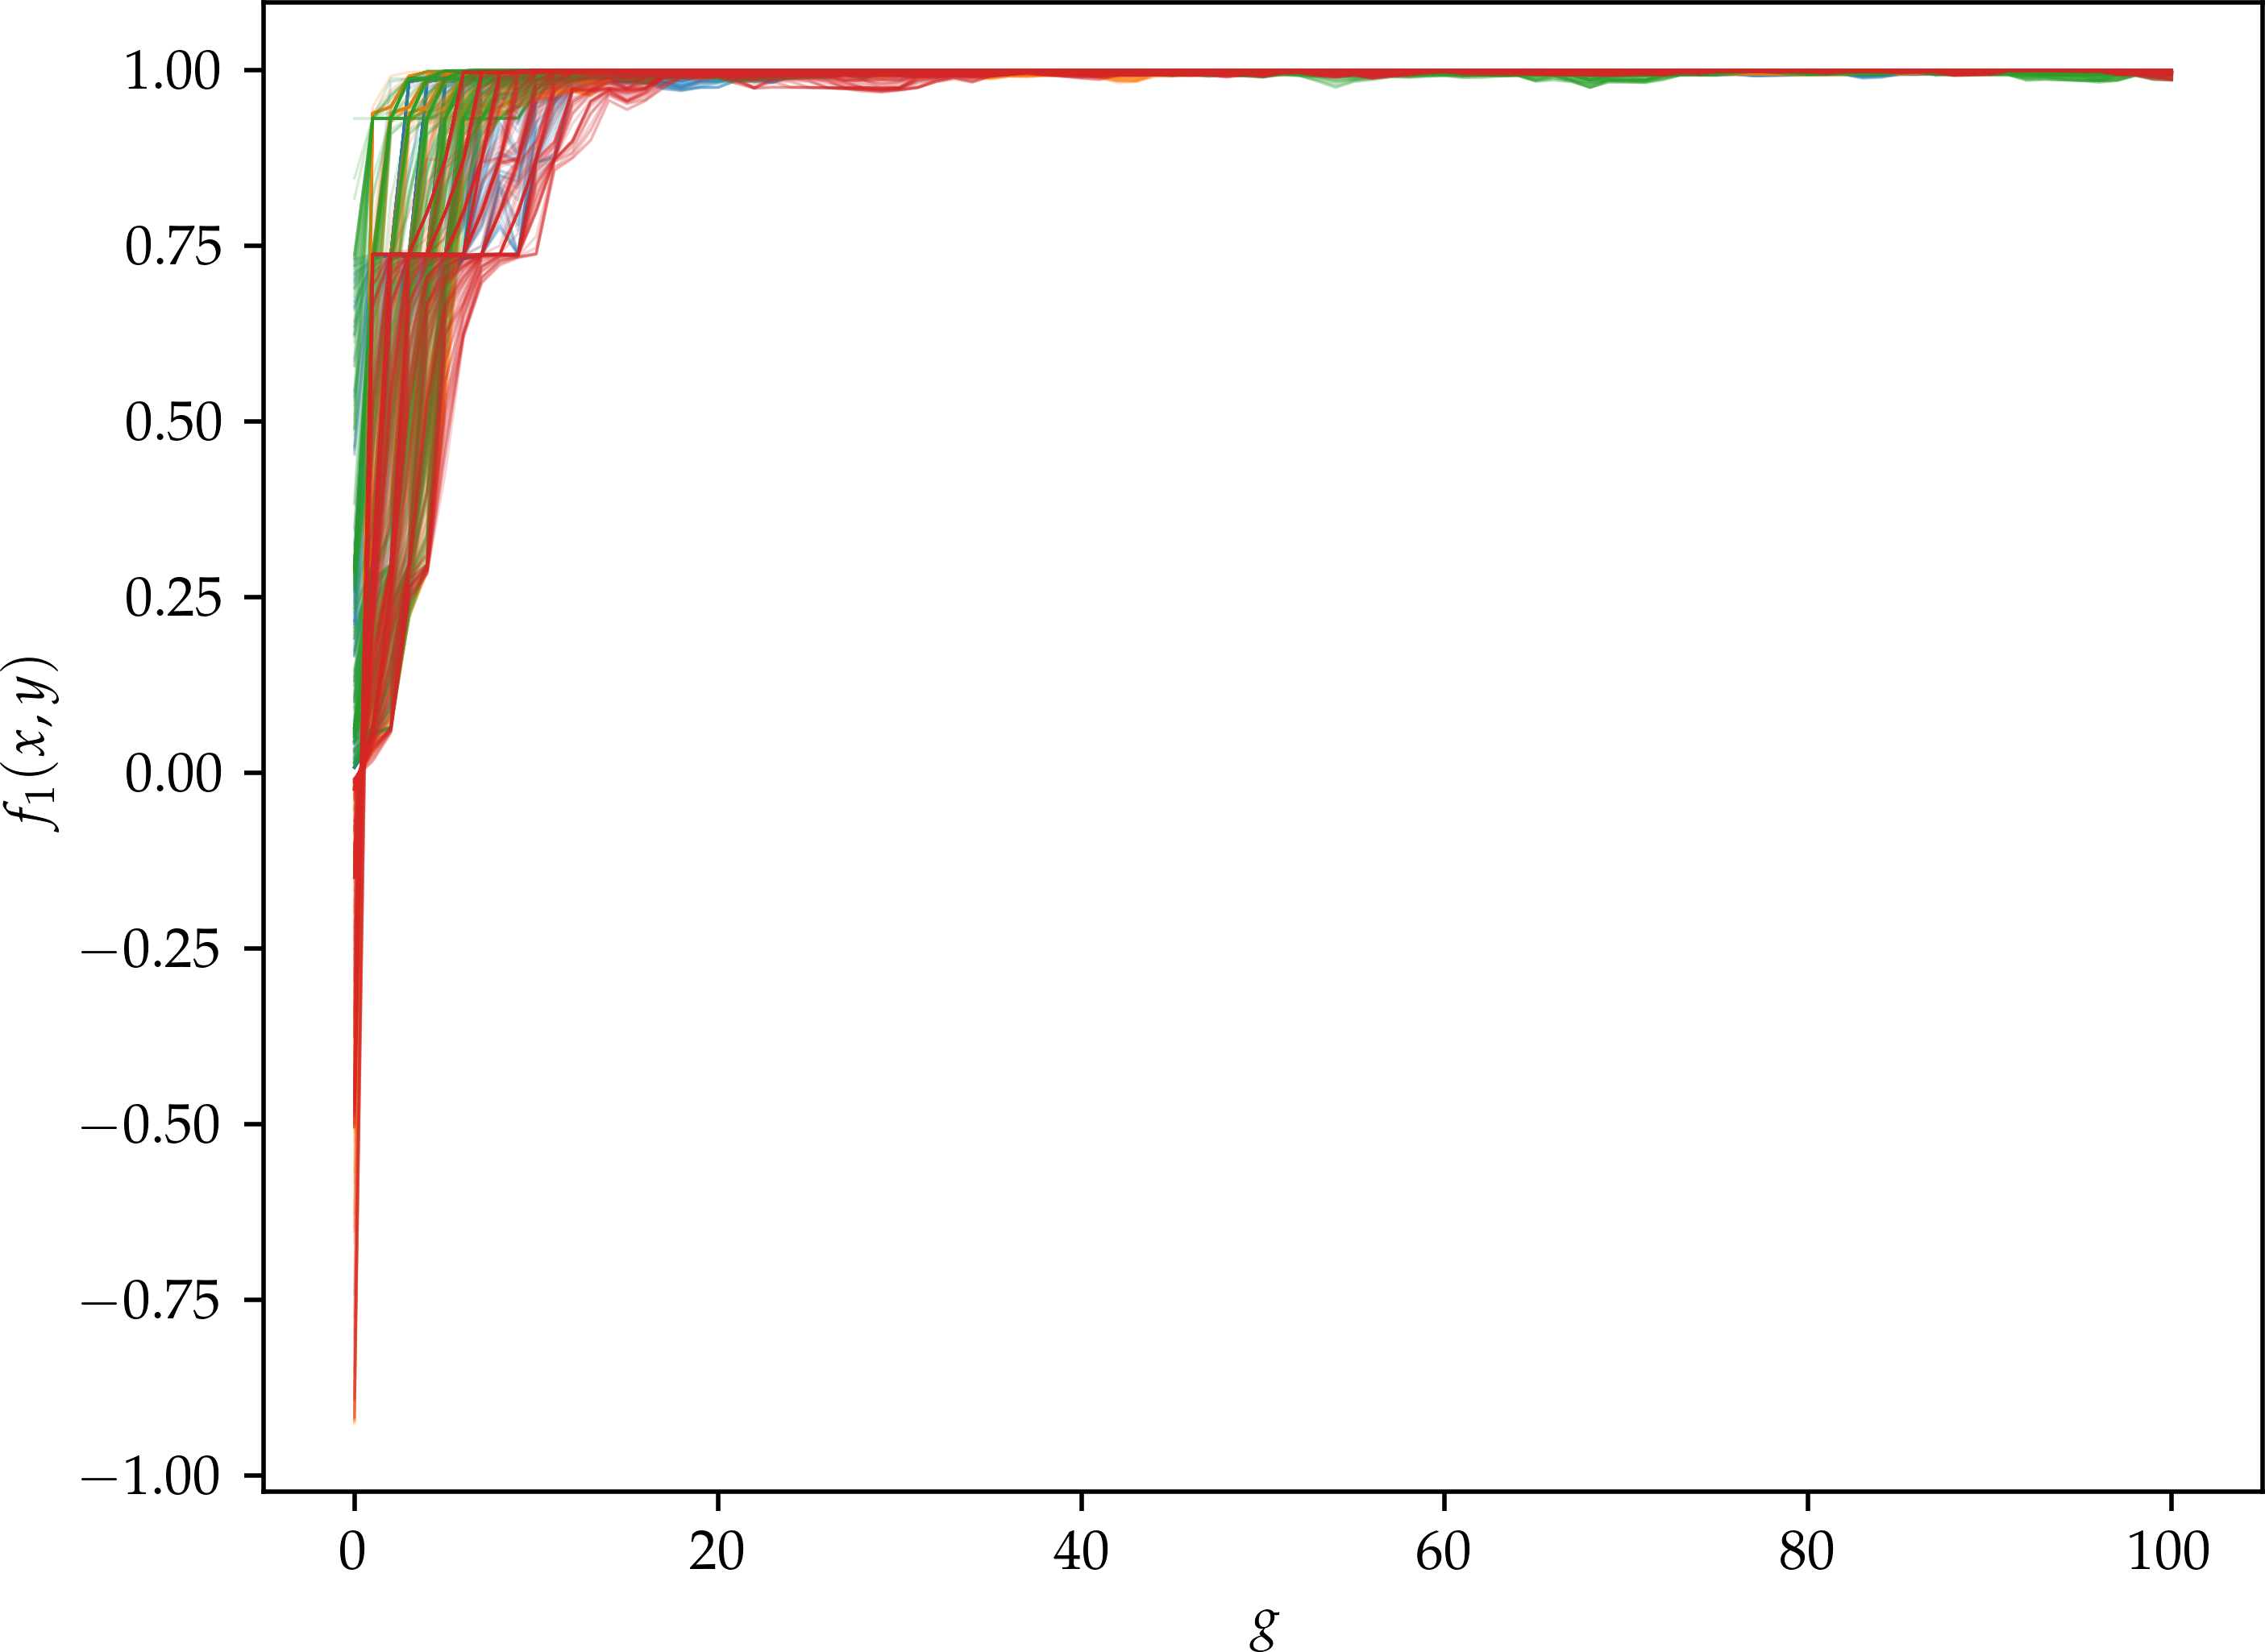
\includegraphics[width=\textwidth]{imagens/low_prob/evolution_damped_cossine.png}
  \caption{
    Evolução dos valores da função $ f_1(x,y) $ para os
    melhores 200 indivíduos de cada população, diferenciadas por cor, em termos da geração $g$,
    com $ p_2 = p_3 = 5\% $.
  }
  \label{fig:evolution_damped_cossine}
\end{figure}

\begin{figure}[p]
  \centering
  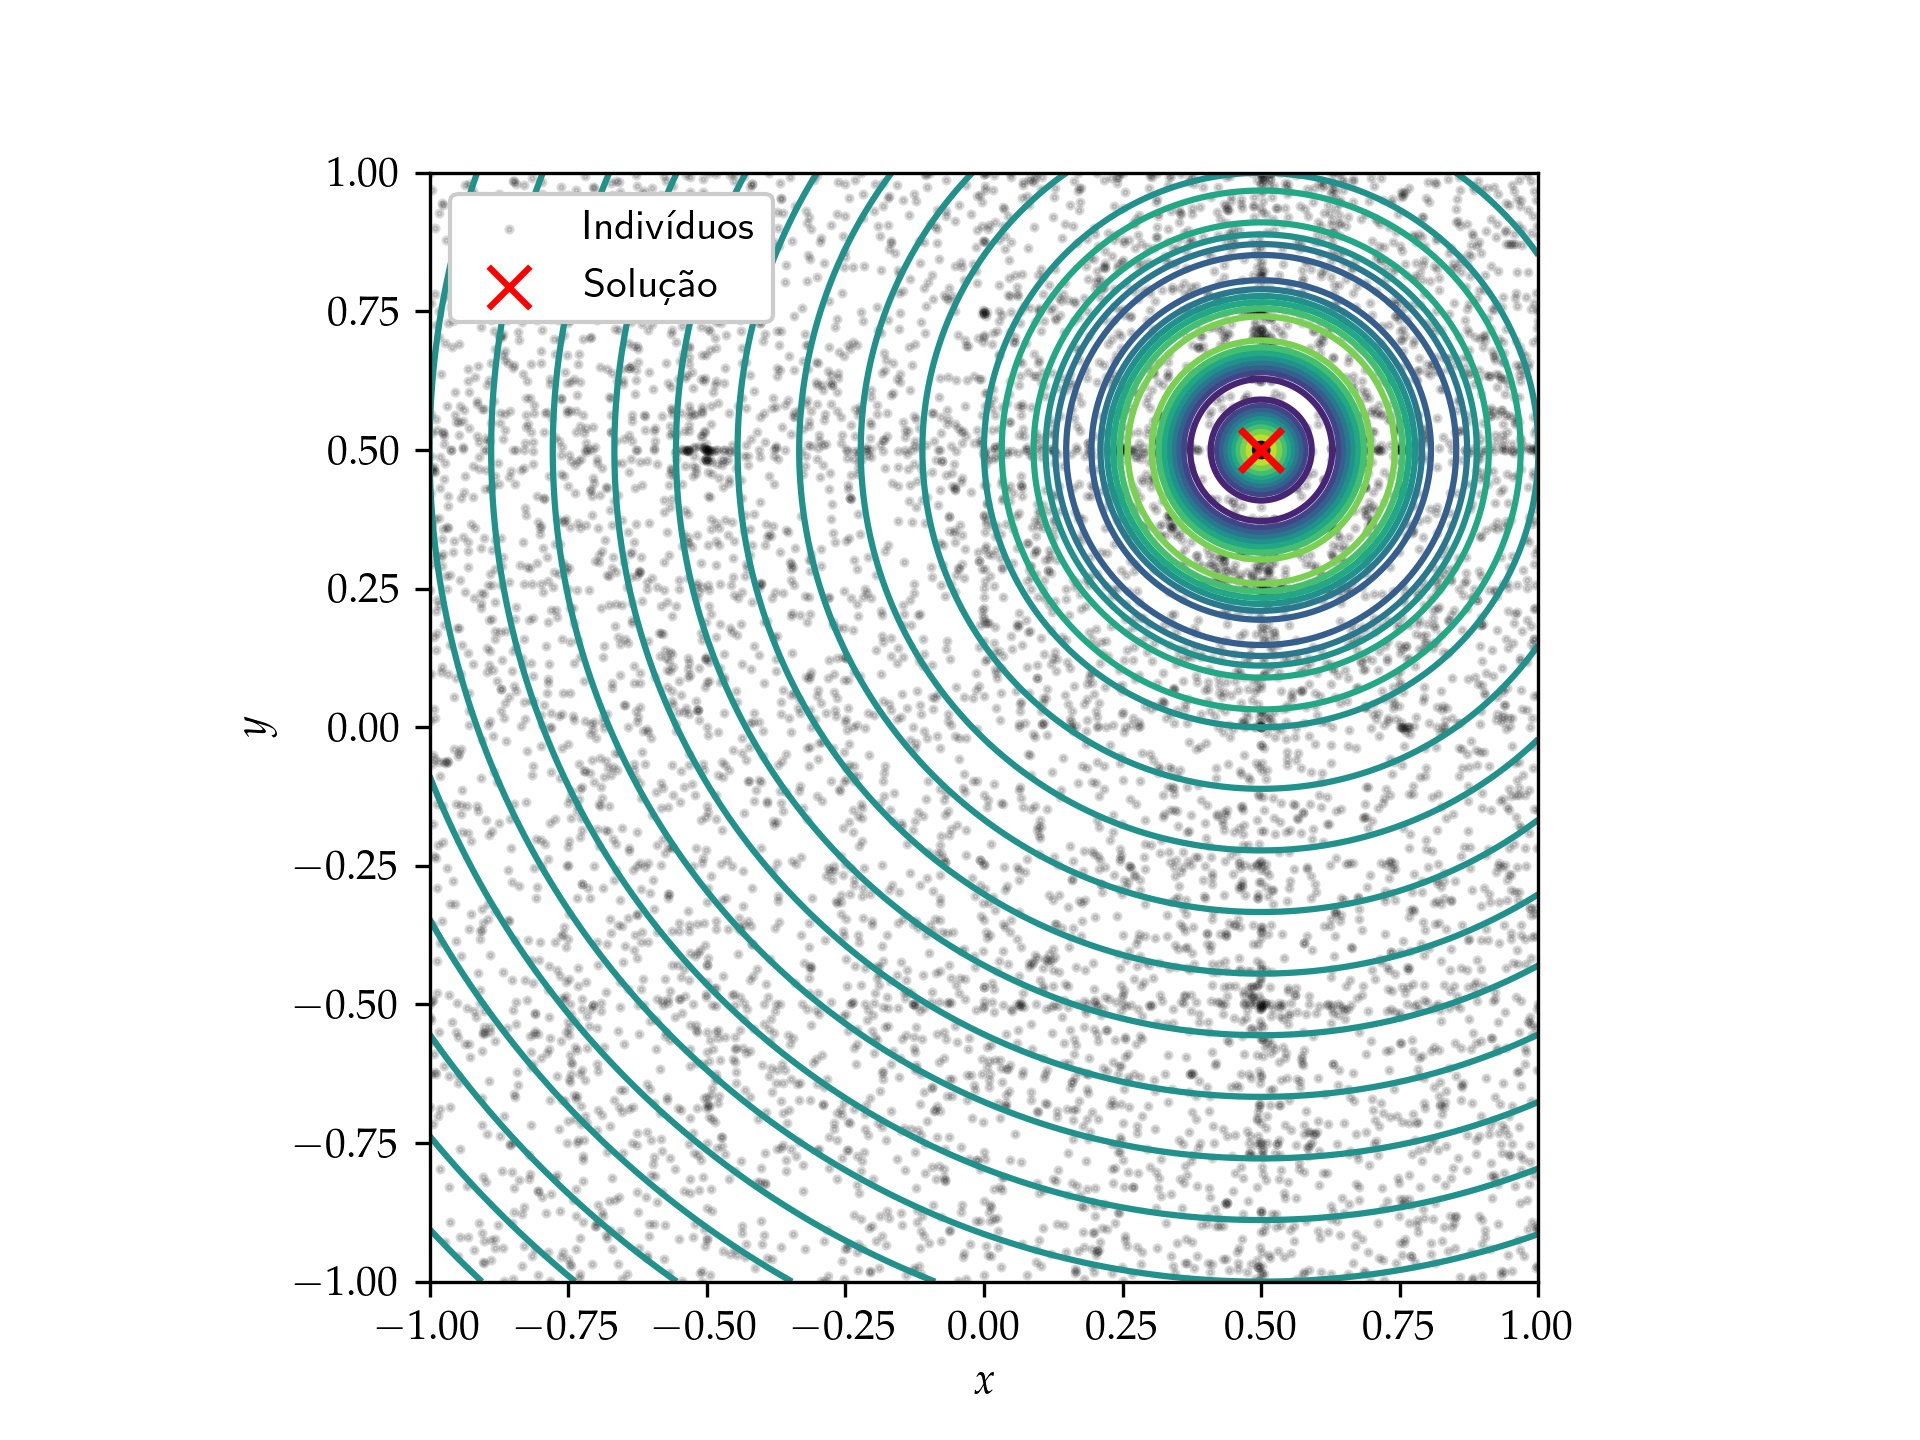
\includegraphics[width=\textwidth]{imagens/high_prob/contour_damped_cossine.png}
  \caption{
    Curvas de nível da função $f_1(x,y)$. Os pontos em preto indicam as posições dos indivíduos
    de 8 populações em sua 100ª geração na otimização da função, com $ p_2 = p_3 = 20\% $. 
    Marcado com um $\times$ vermelho estão os melhores indivíduos de cada população.
  }
  \label{fig:contour_damped_cossine_mut_20}
\end{figure}

\begin{figure}[p]
  \centering
  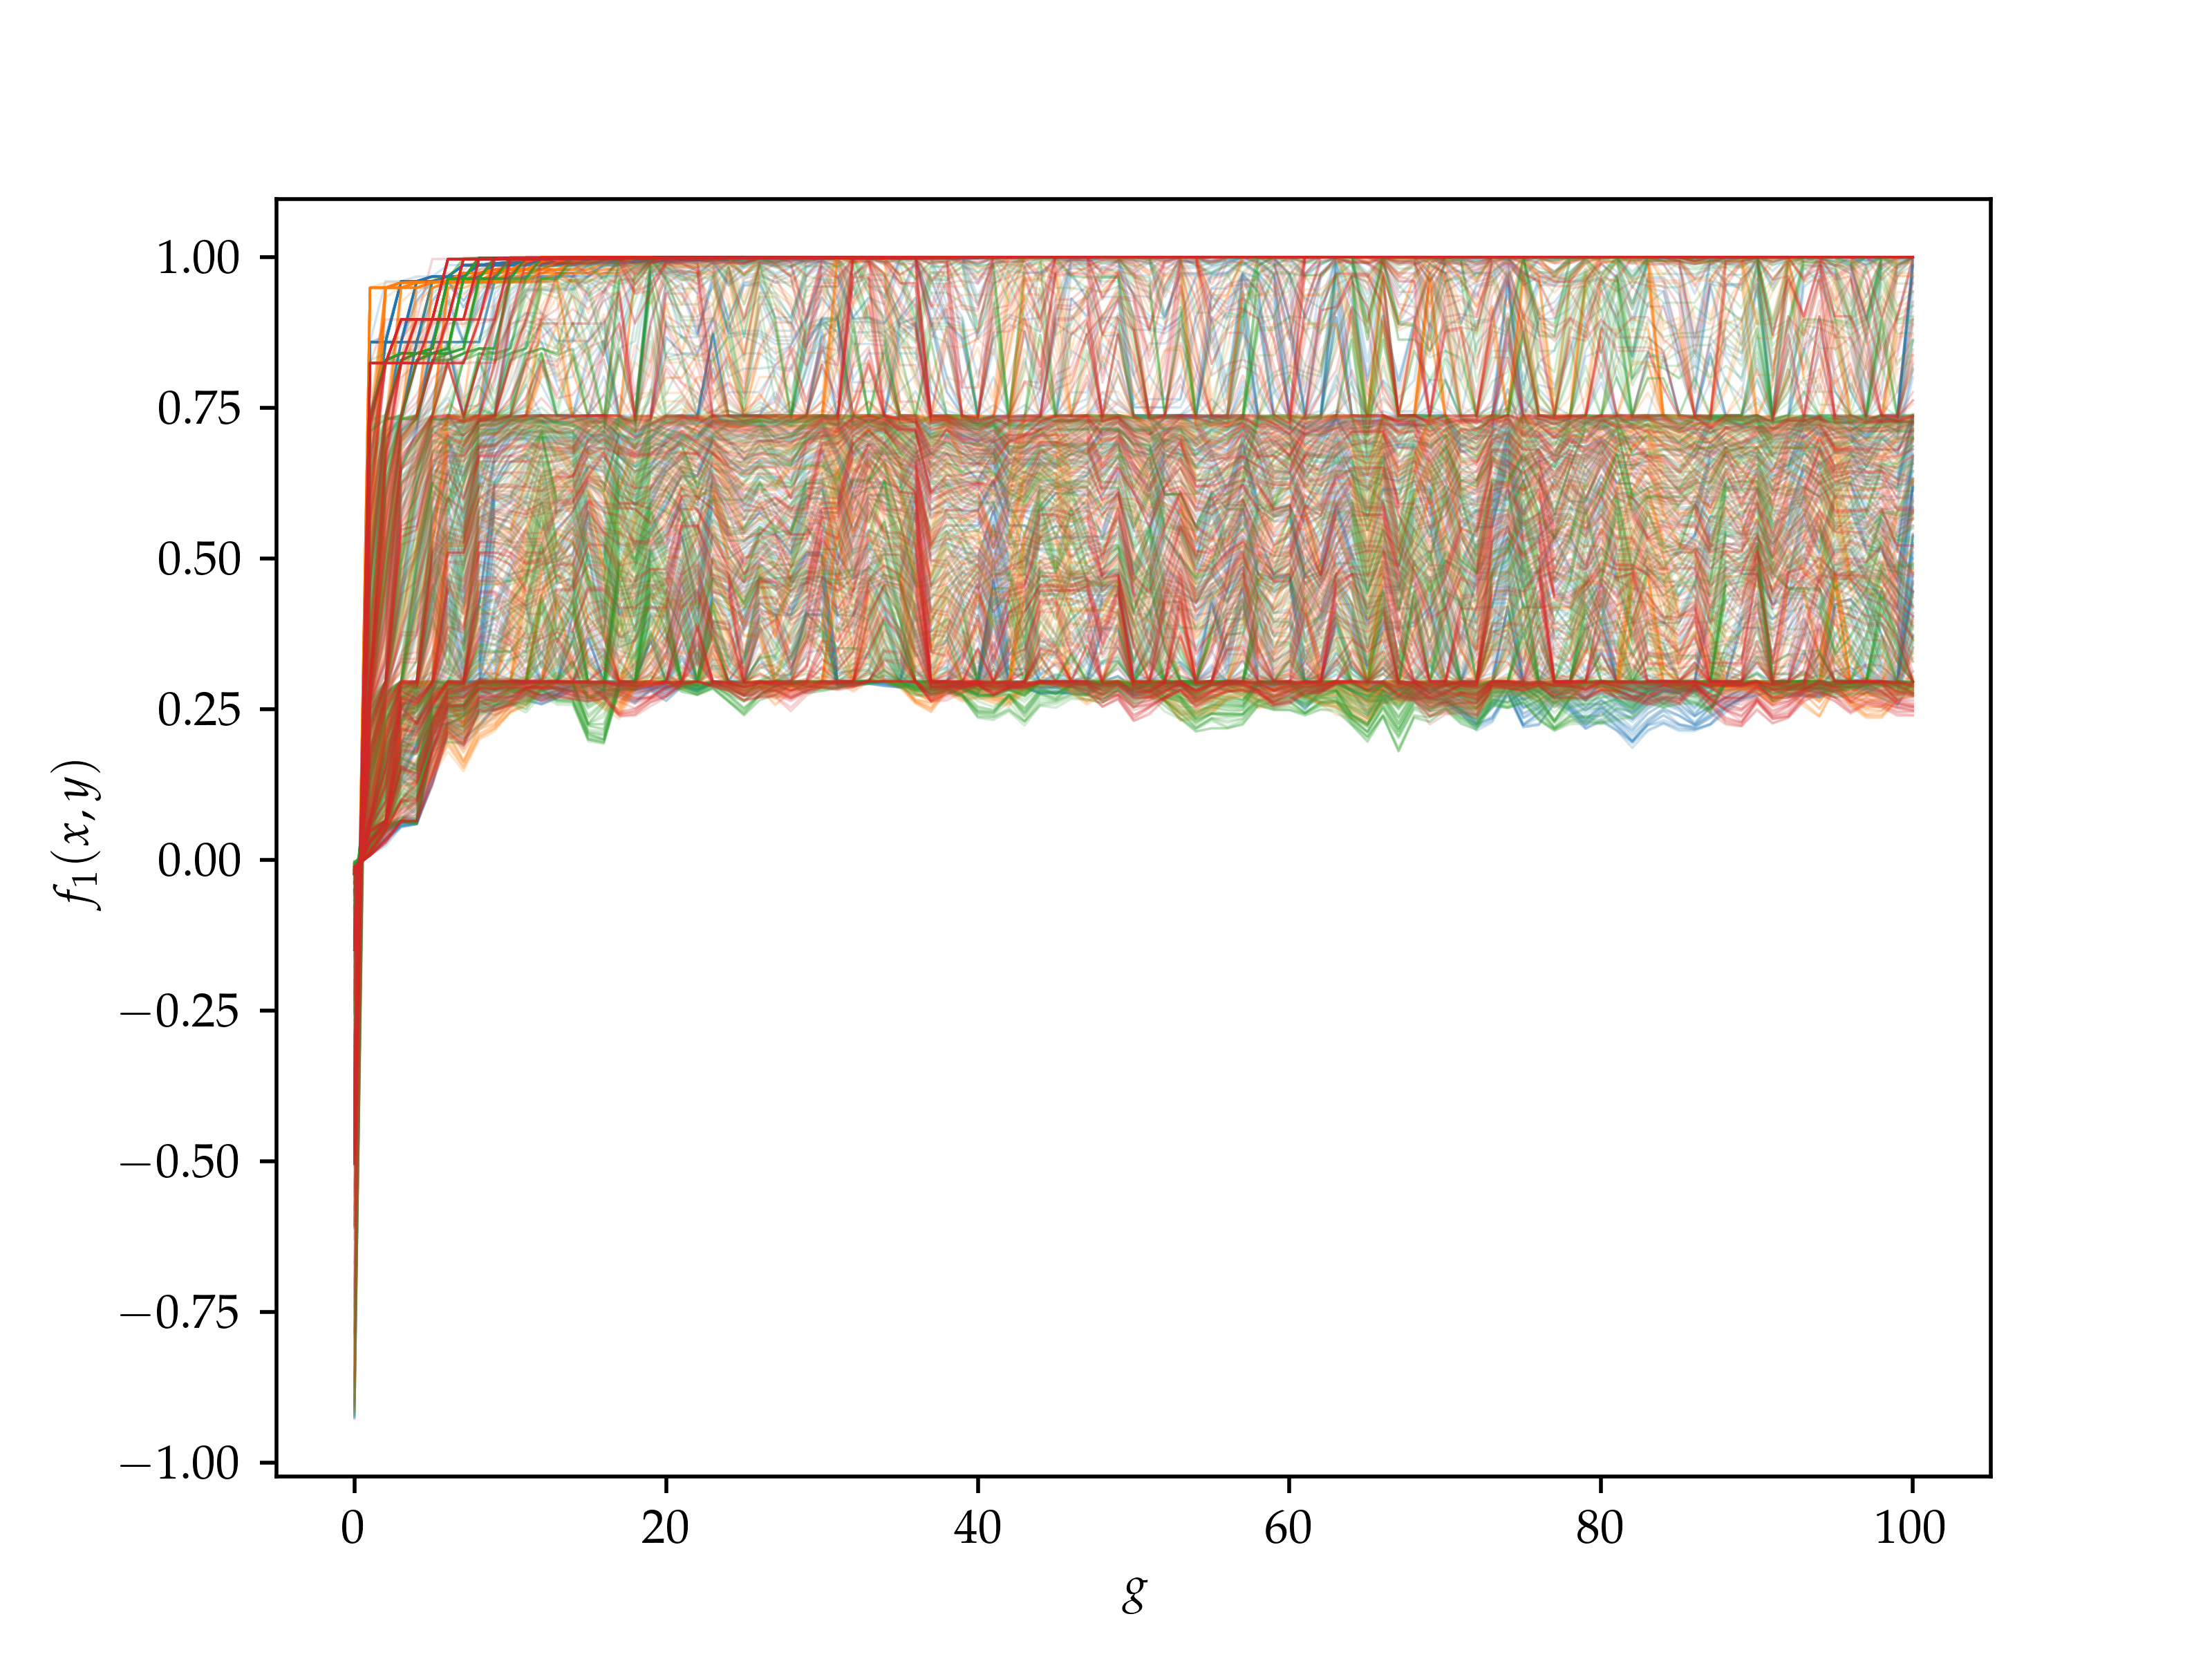
\includegraphics[width=\textwidth]{imagens/high_prob/evolution_damped_cossine.png}
  \caption{
    Evolução dos valores da função $ f_1(x,y) $ para os
    melhores 200 indivíduos de cada população, diferenciadas por cor, em termos da geração $g$,
    com $ p_2 = p_3 = 20\% $.
  }
  \label{fig:evolution_damped_cossine_mut_20}
\end{figure}

\begin{figure}[p]
  \centering
  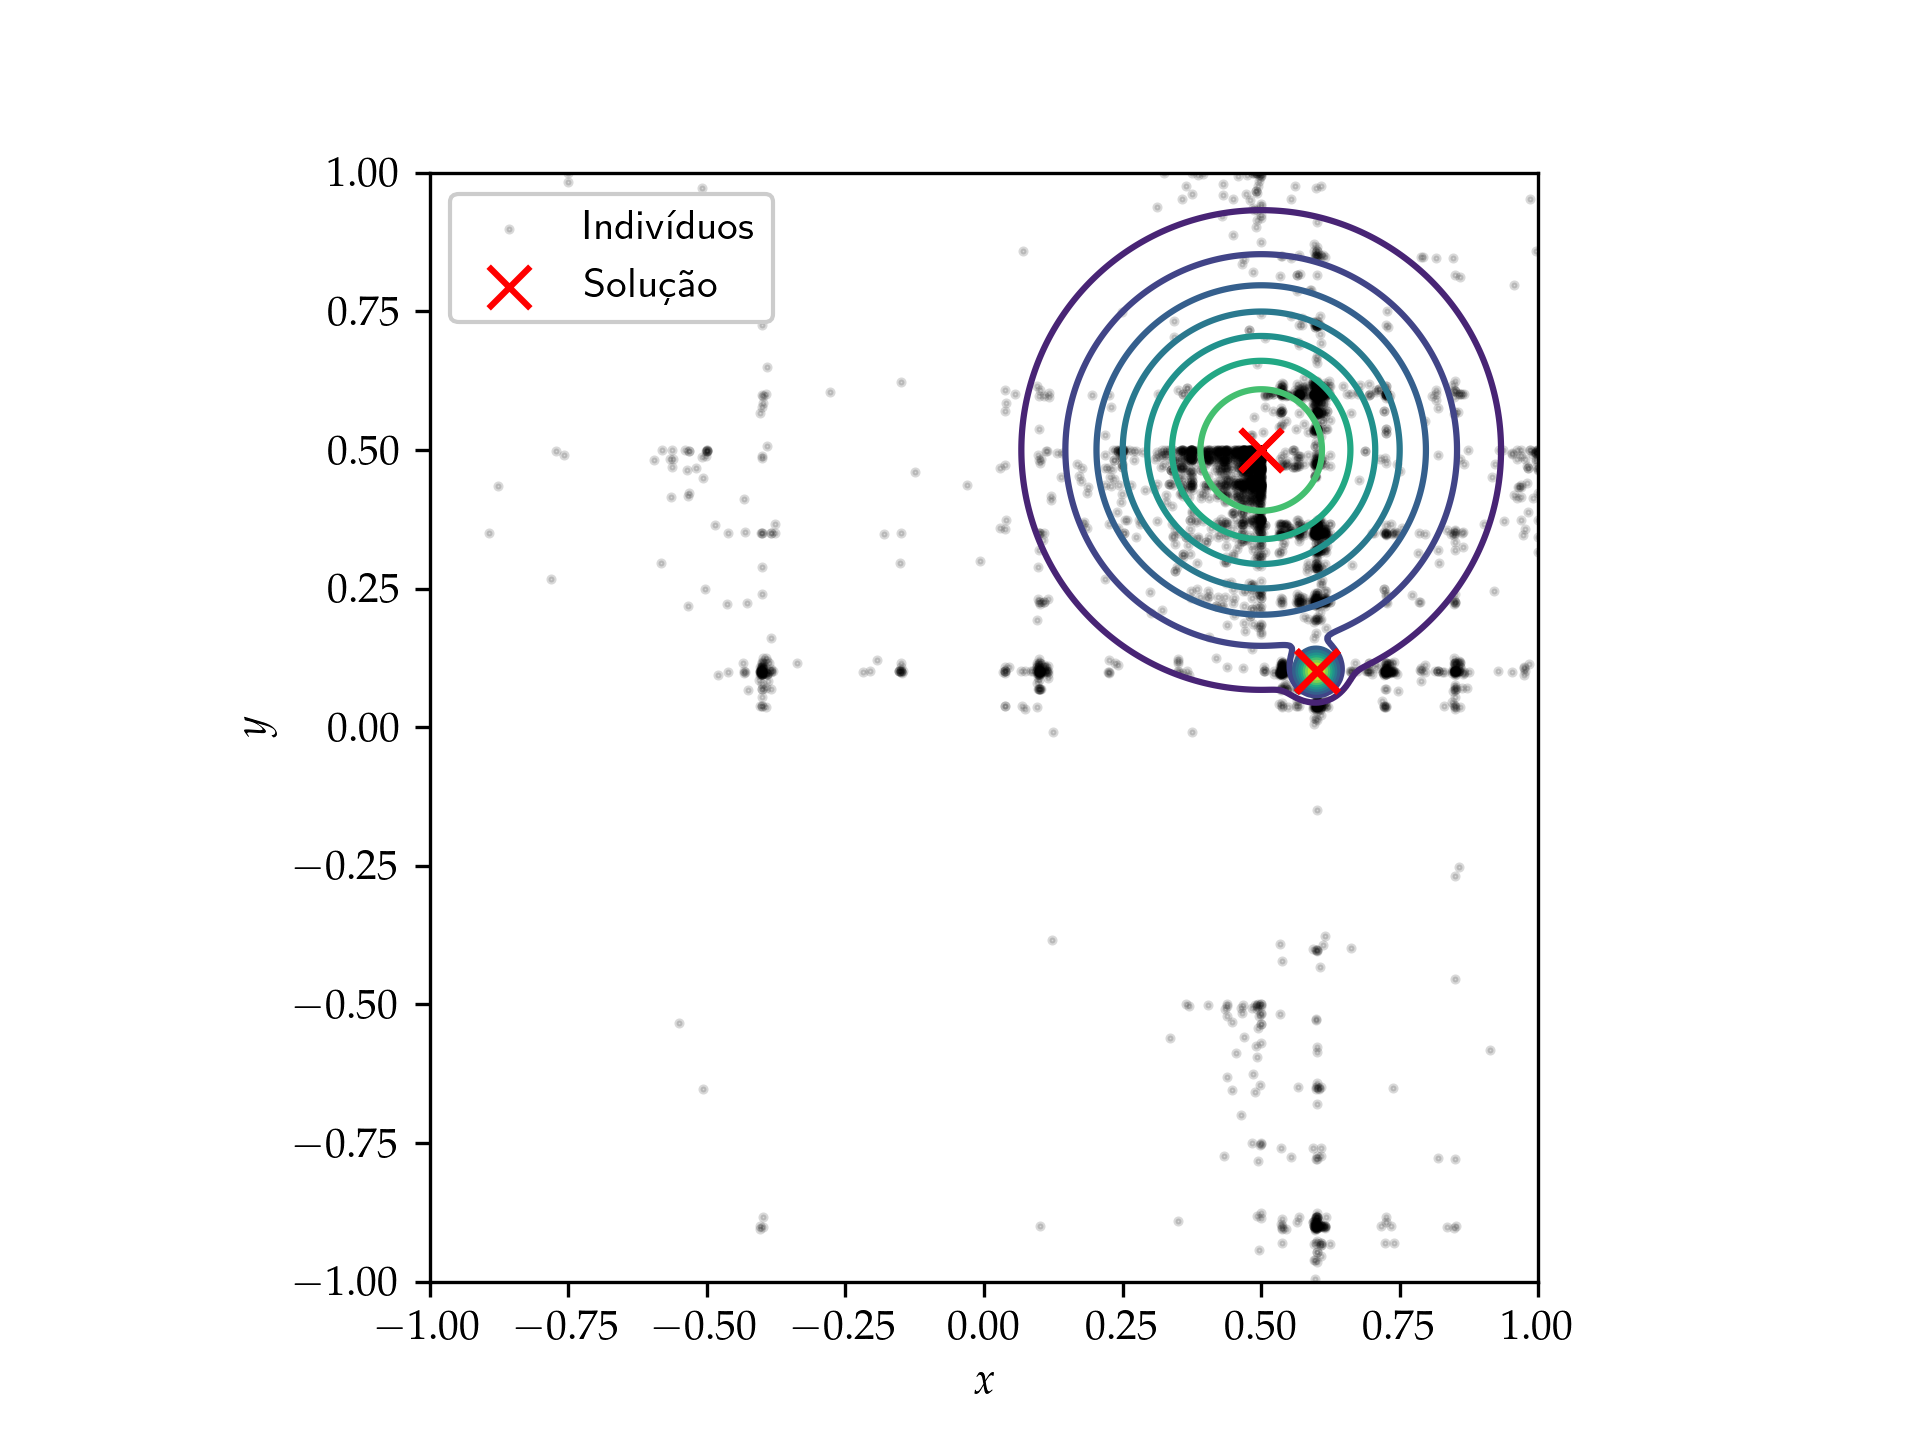
\includegraphics[width=\textwidth]{imagens/low_prob/contour_near_gaussians.png}
  \caption{
    Curvas de nível da função $f_2(x,y)$. Os pontos em preto indicam as posições dos indivíduos
    de 8 populações em sua 100ª geração na otimização da função, com $ p_2 = p_3 = 5\% $. 
    Marcado com um $\times$ vermelho estão os melhores indivíduos de cada população.
  }
  \label{fig:contour_near_gaussians}
\end{figure}

\begin{figure}[p]
  \centering
  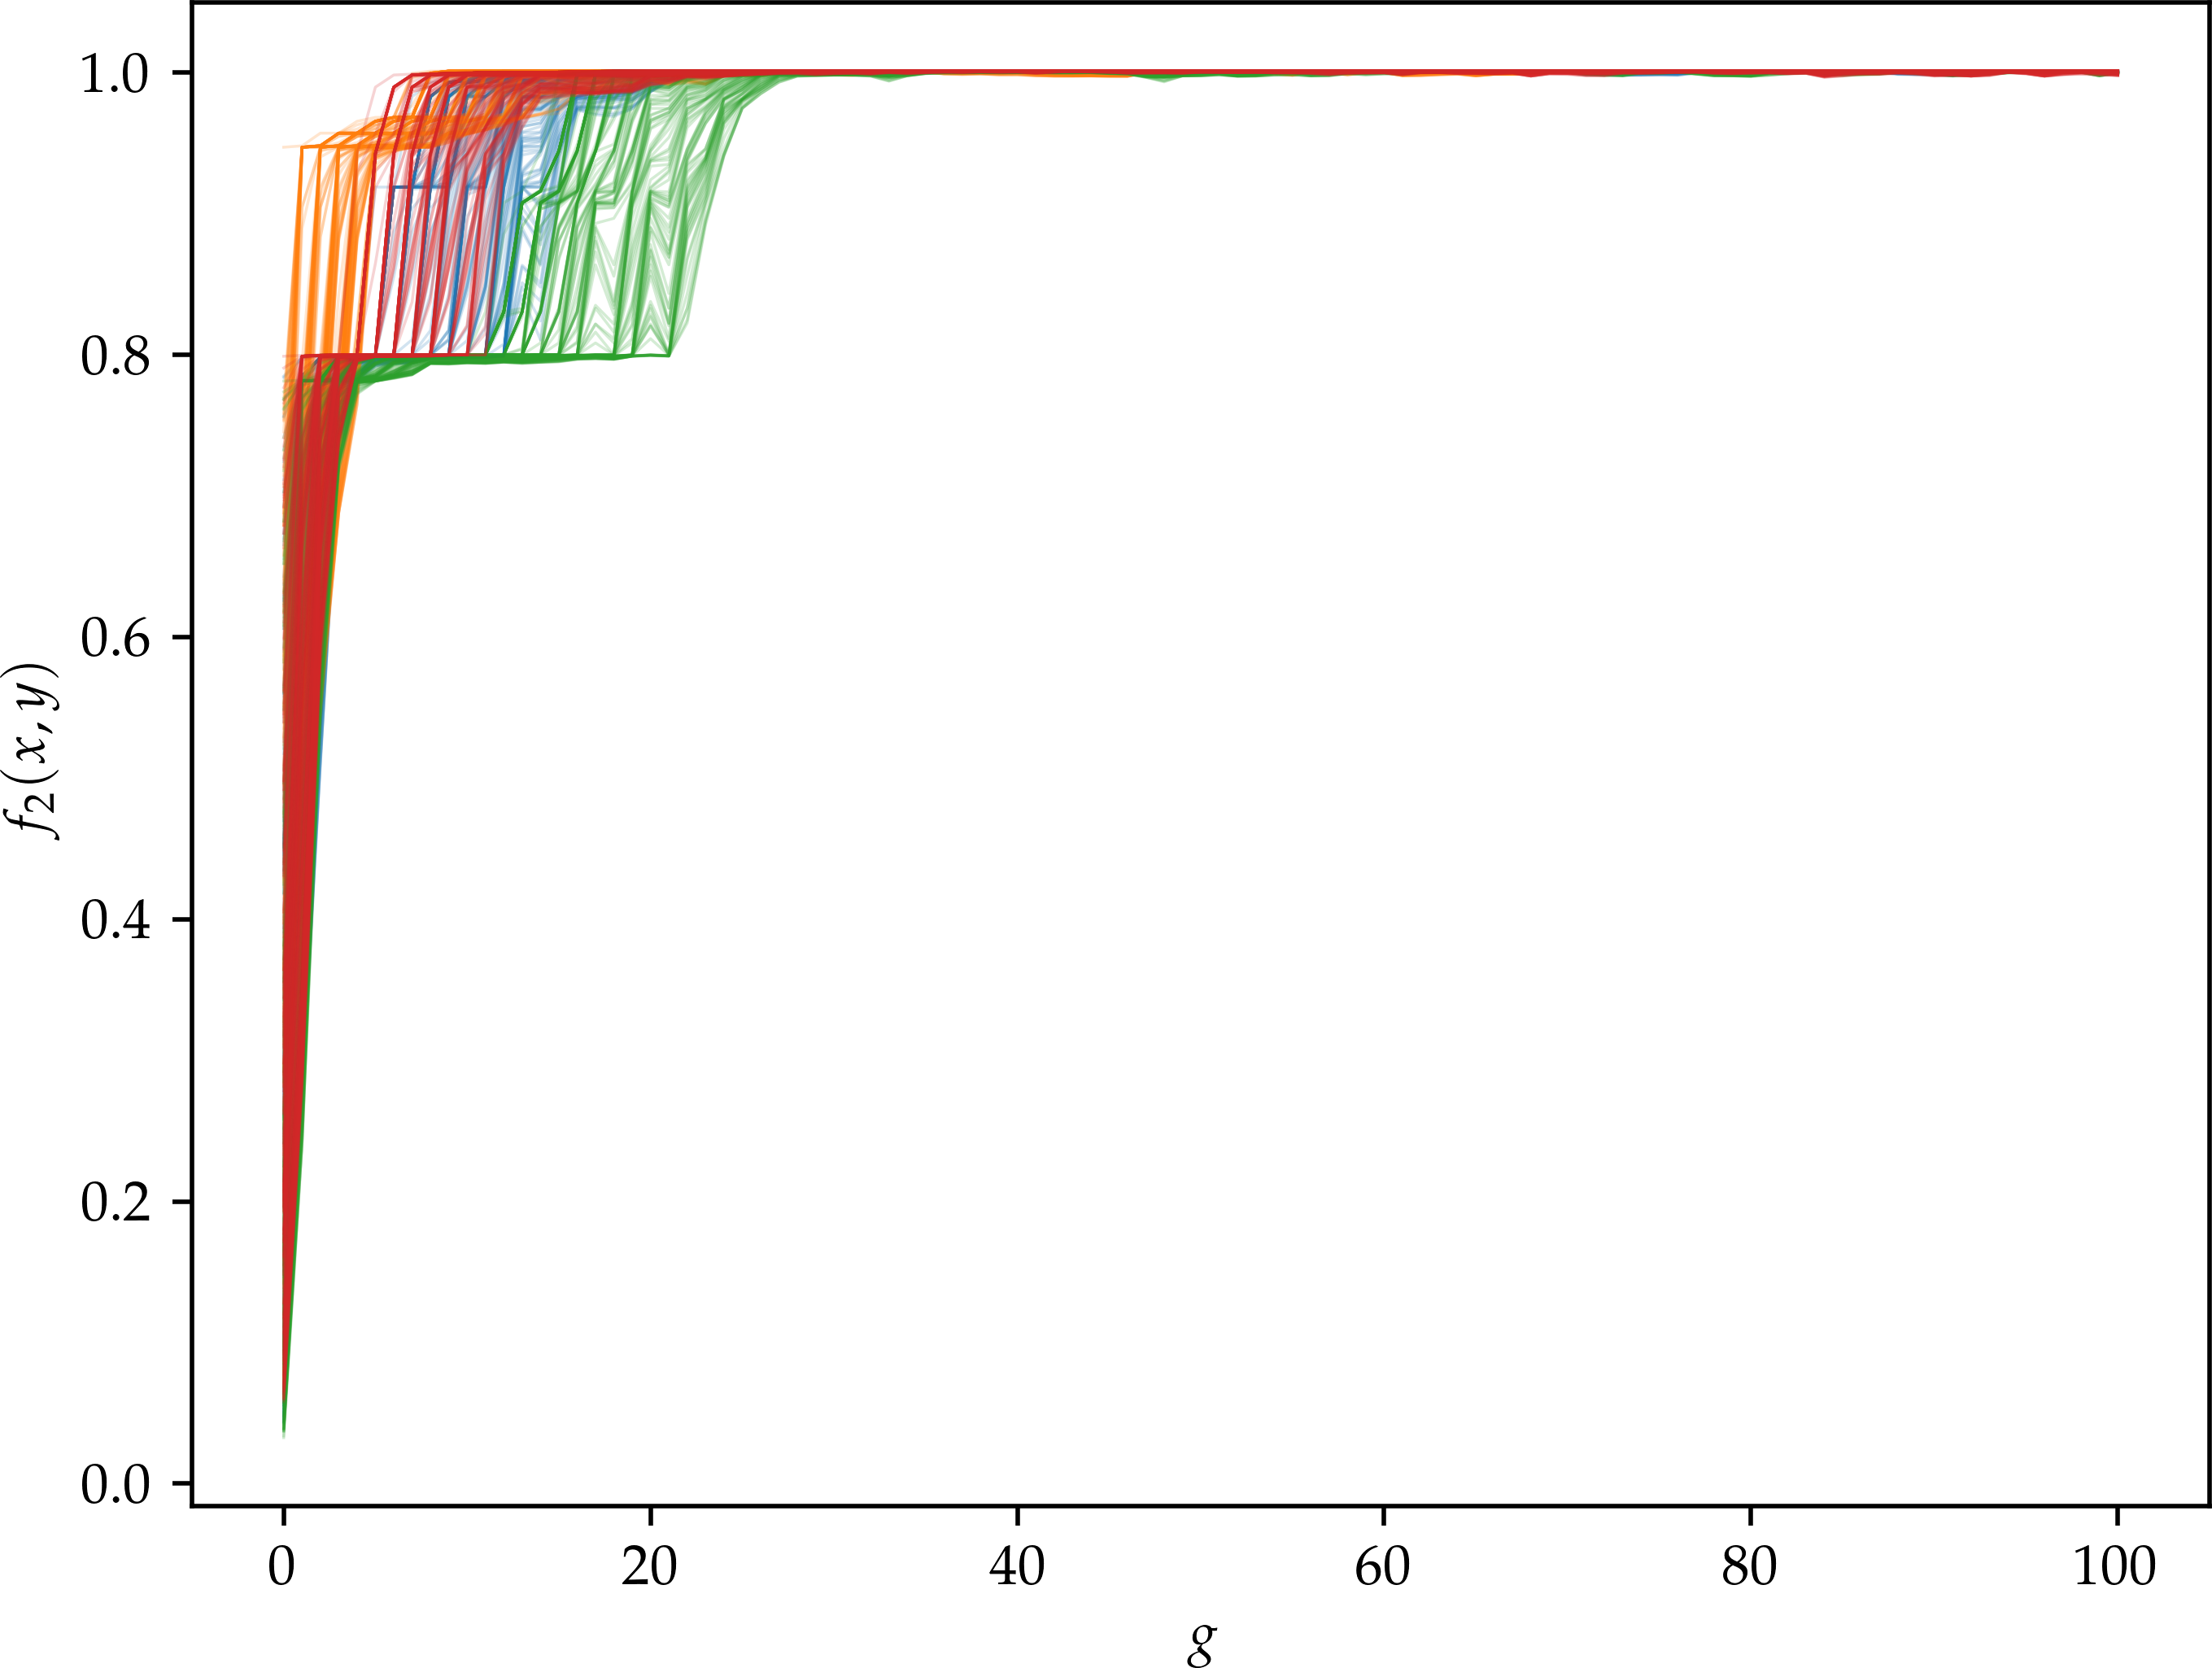
\includegraphics[width=\textwidth]{imagens/low_prob/evolution_near_gaussians.png}
  \caption{
    Evolução dos valores da função $ f_2(x,y) $ para os
    melhores 200 indivíduos de cada população, diferenciadas por cor, em termos da geração $g$,
    com $ p_2 = p_3 = 5\% $.
  }
  \label{fig:evolution_near_gaussians}
\end{figure}

\begin{figure}[p]
  \centering
  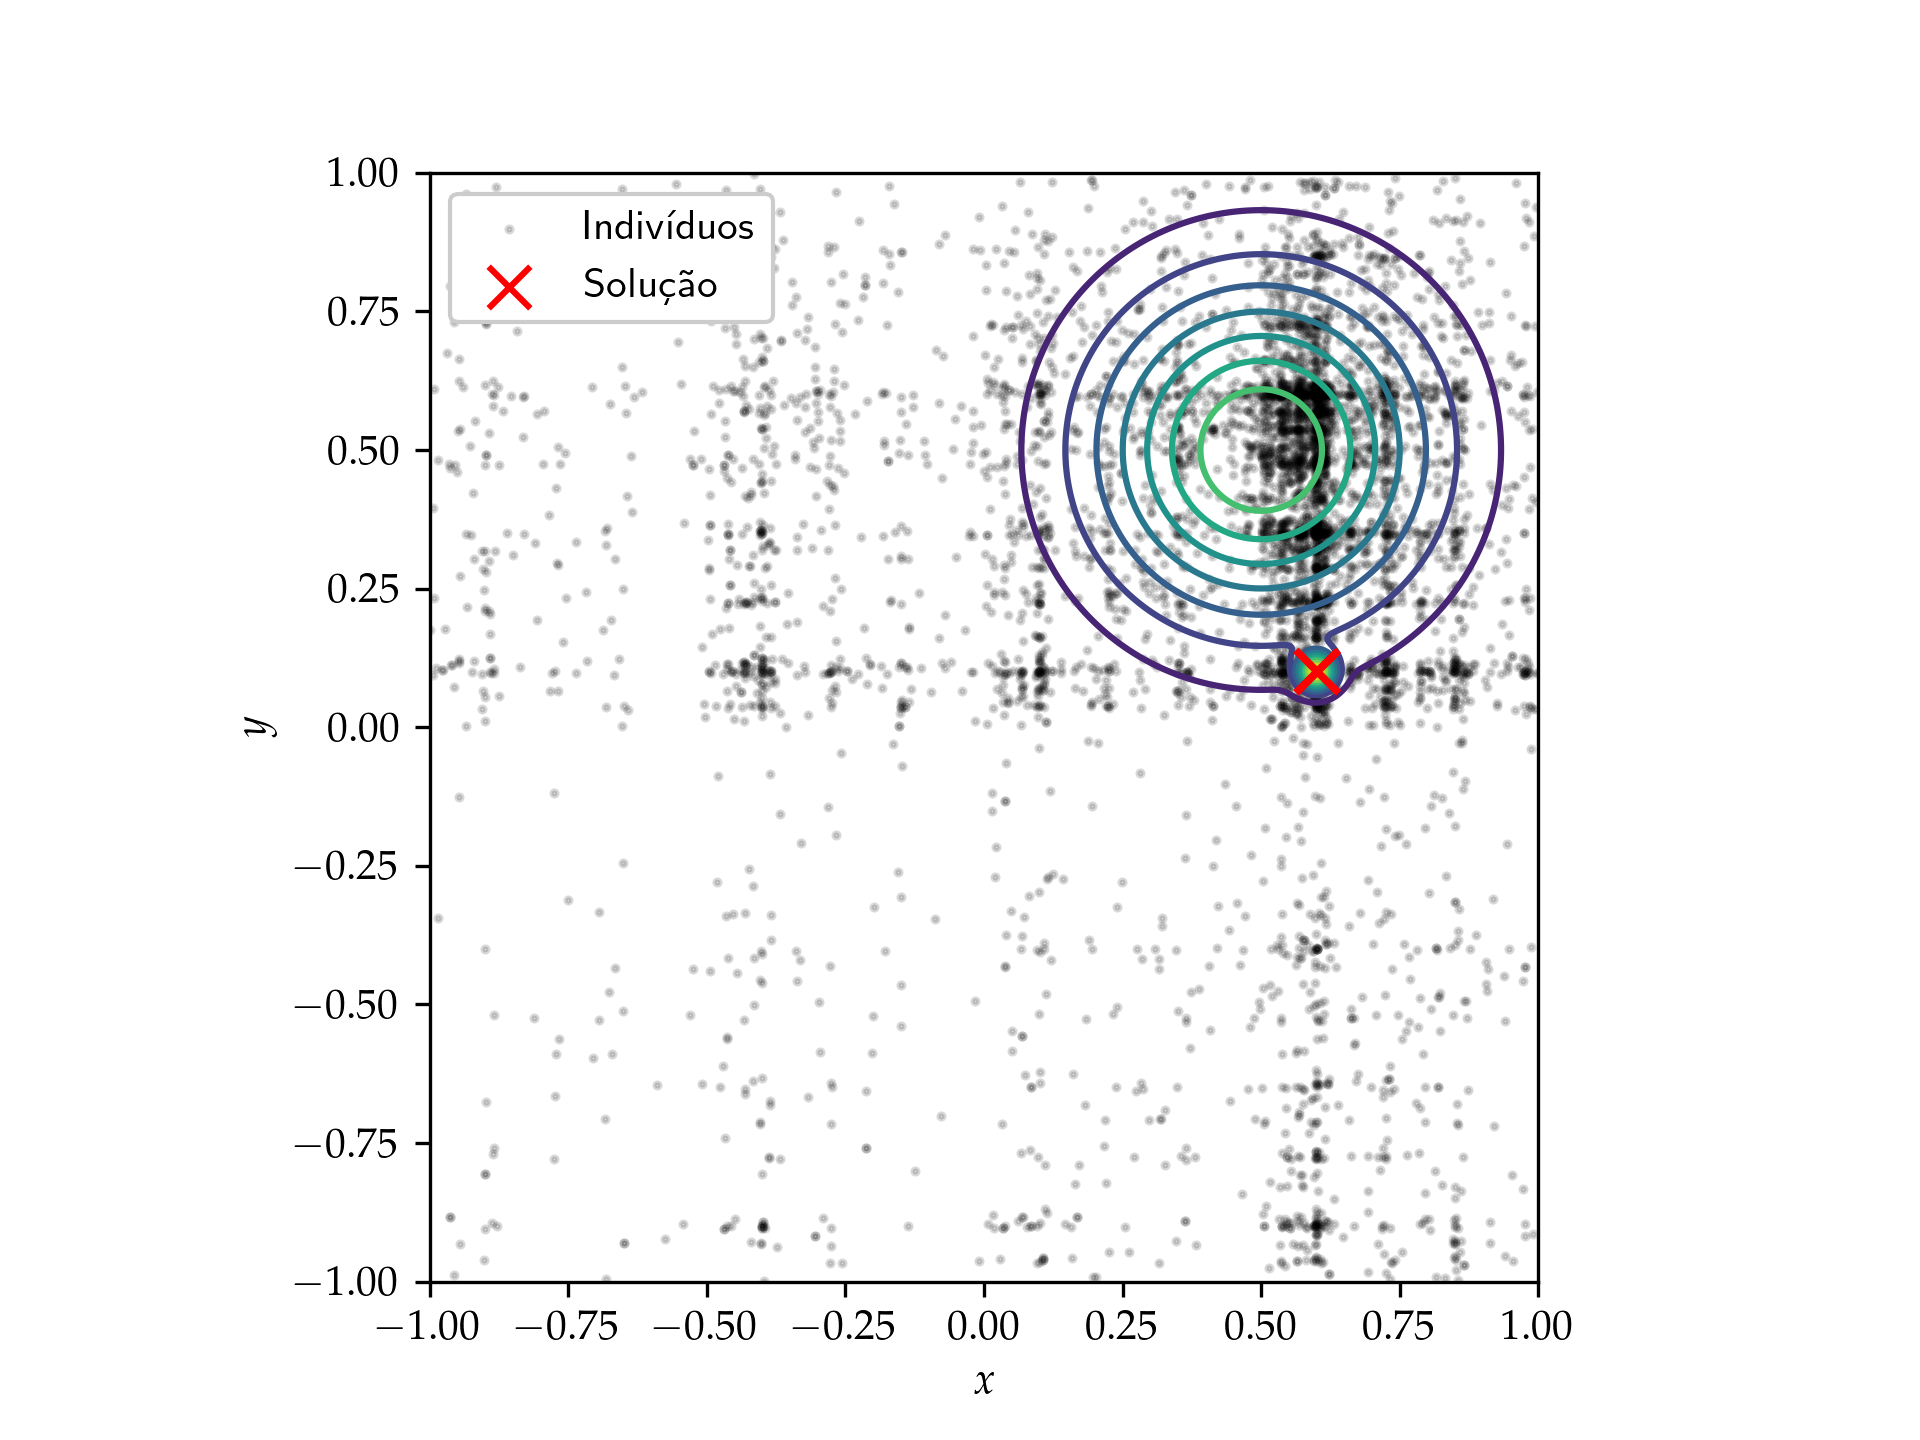
\includegraphics[width=\textwidth]{imagens/high_prob/contour_near_gaussians.png}
  \caption{
    Curvas de nível da função $f_2(x,y)$. Os pontos em preto indicam as posições dos indivíduos
    de 8 populações em sua 100ª geração na otimização da função, com $ p_2 = p_3 = 20\% $. 
    Marcado com um $\times$ vermelho estão os melhores indivíduos de cada população.
  }
  \label{fig:contour_near_gaussians_mut_20}
\end{figure}

\begin{figure}[p]
  \centering
  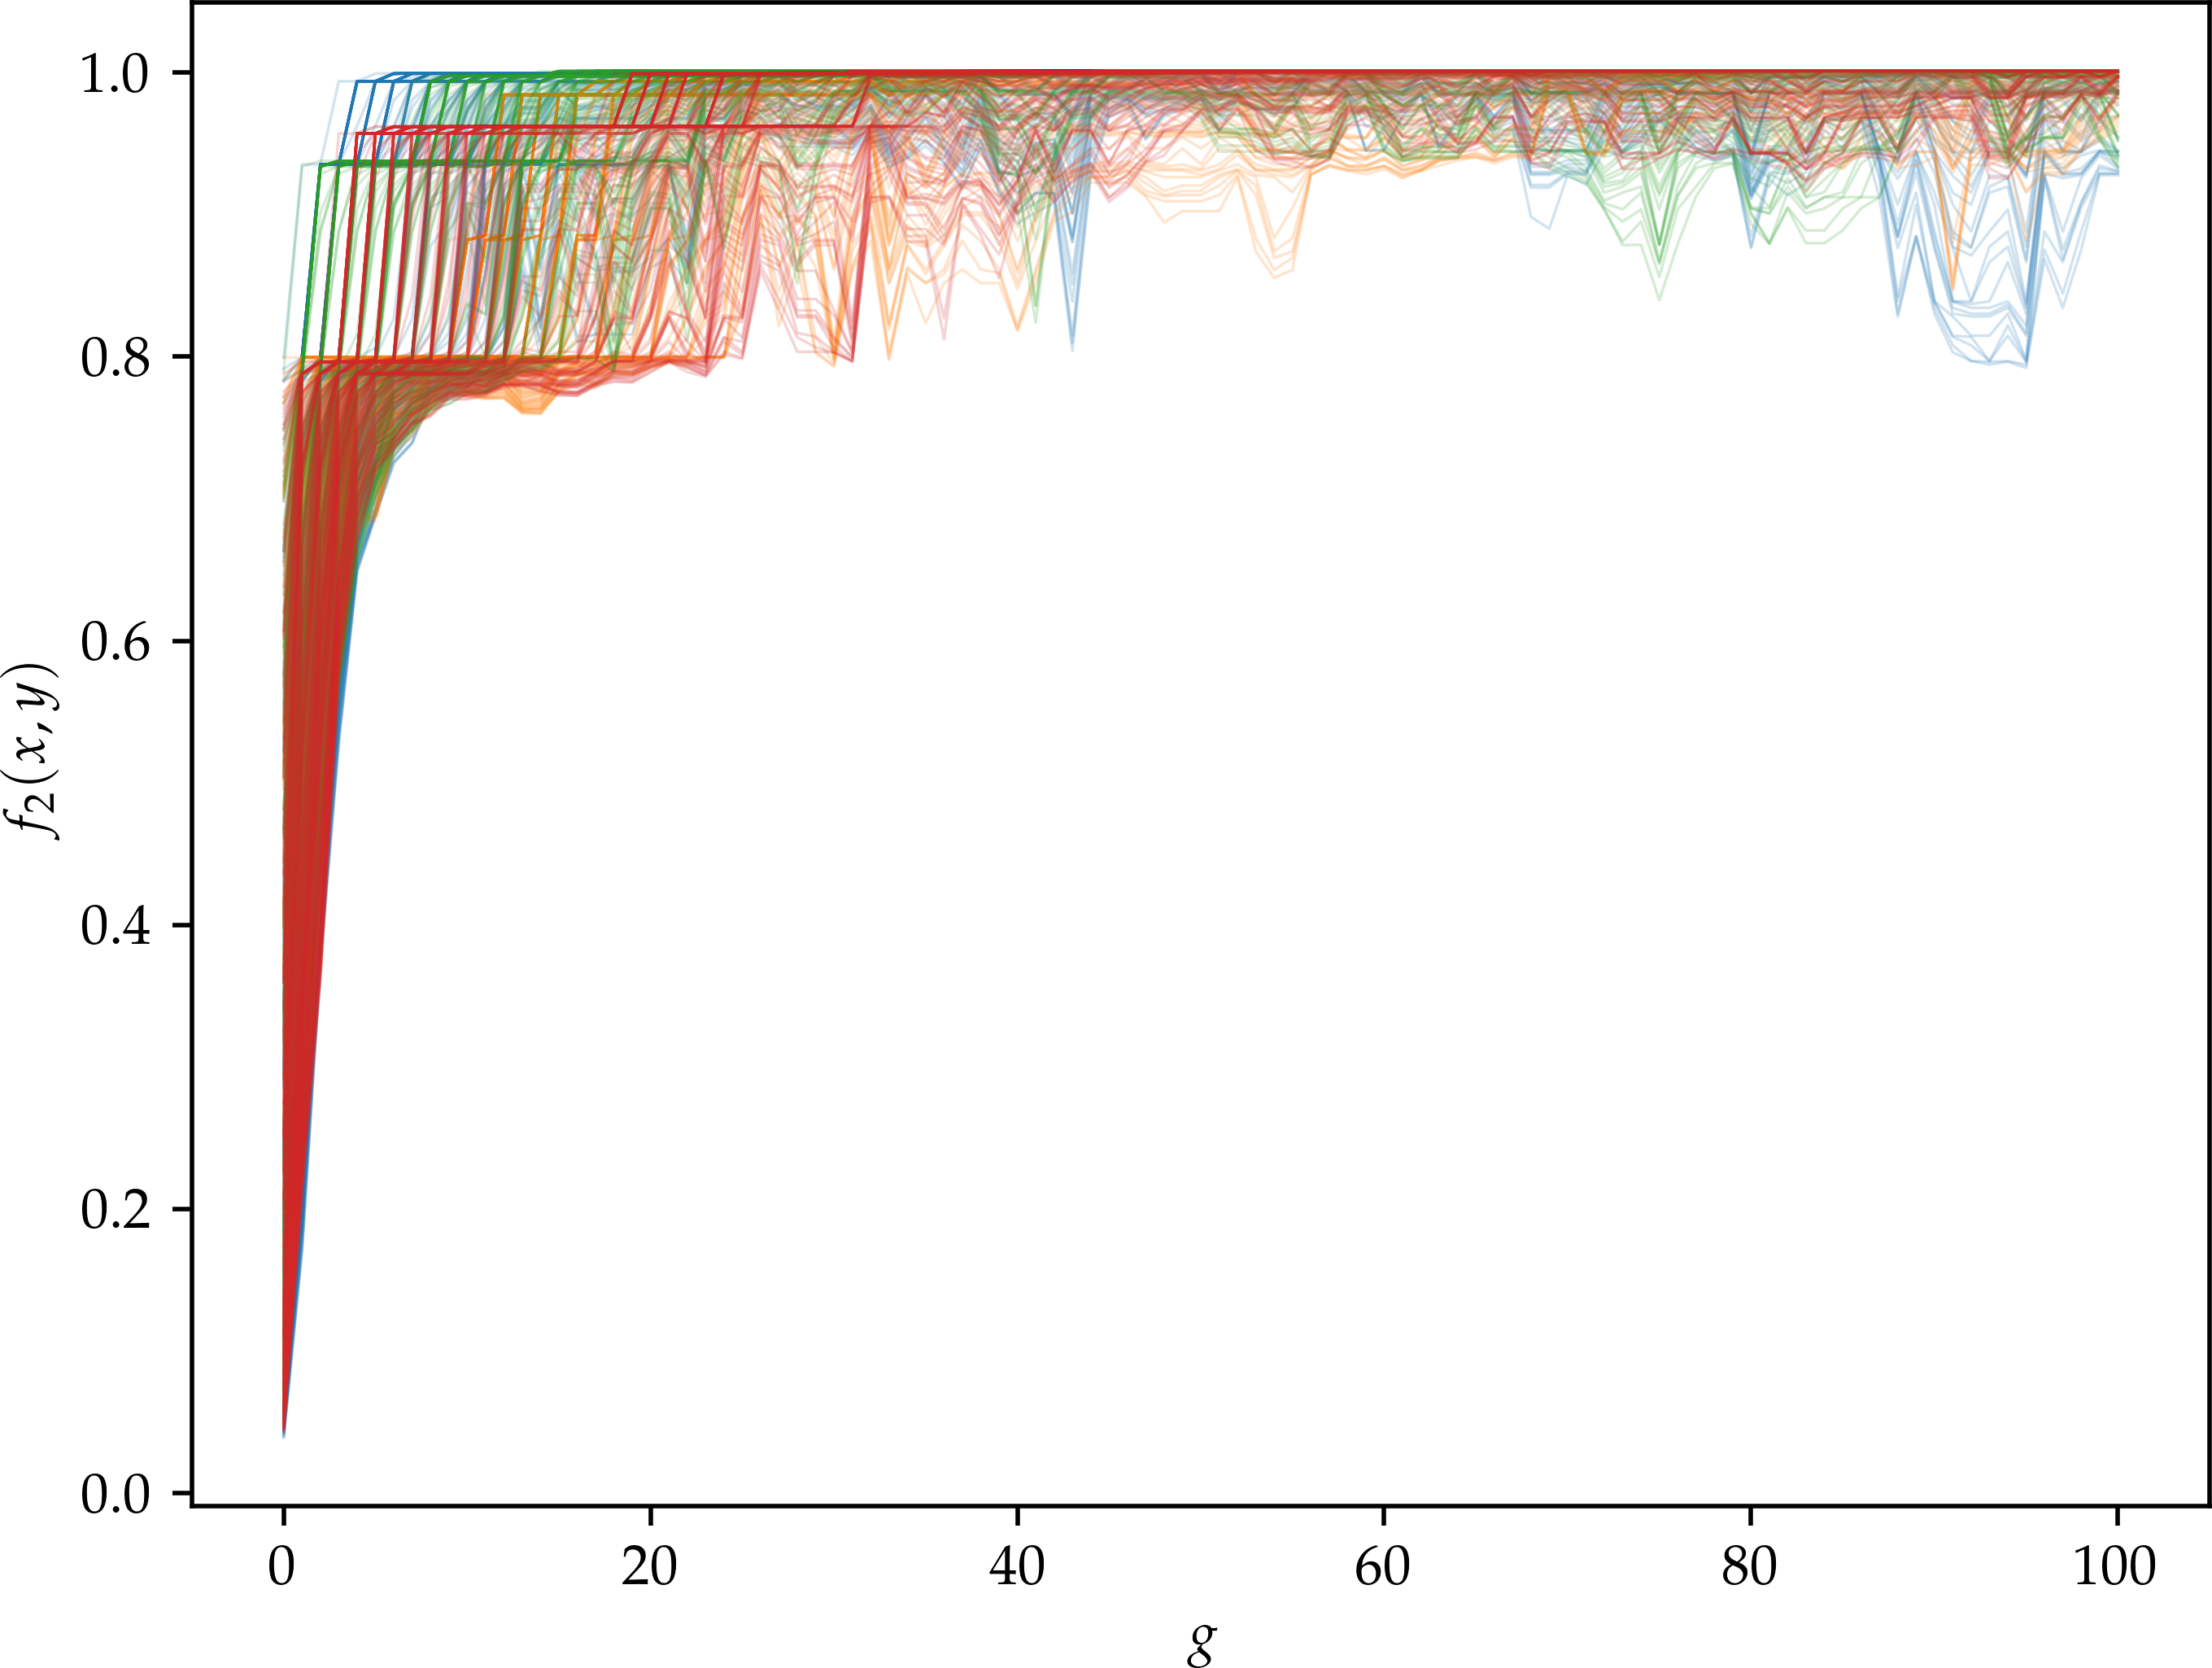
\includegraphics[width=\textwidth]{imagens/high_prob/evolution_near_gaussians.png}
  \caption{
    Evolução dos valores da função $ f_2(x,y) $ para os
    melhores 200 indivíduos de cada população, diferenciadas por cor, em termos da geração $g$,
    com $ p_2 = p_3 = 20\% $.
  }
  \label{fig:evolution_near_gaussians_mut_20}
\end{figure}

\section{Ajuste das Estruturas de Banda dos Cristais \ch{CrS2} e \ch{CrSe2}}
\label{sec_resultados_tmdcs}

Para o ajuste das bandas de energia dos materiais \ch{CrS2} e \ch{CrSe2} foram
executados 16 processos simultâneos com 1000 indivíduos cada, evoluídos no
decorrer de 100 gerações, com probabilidades de mutação $ p_2 = p_3 = 5\% $ e
$ h = 2 $. A distribuição da elite nas populações ocorreu de forma que $ e_1 =
  5\% $, $ e_2 = e_3 = 10\% $, sendo os percentuais tomados em relação ao tamanho
da população. A região de busca considerada no processo de ajuste é dada pelo
produto cartesiano dos intervalos na Tabela \ref{tab:search_region}.

\begin{table}[h]
  \centering
  \begin{tabular}{lrr}
    \toprule
                & $\xmin{j}$ & $\xmax{j}$ \\
    \midrule
    $E_F$       & \num{-1.0} & \num{1.0}  \\
    $\Delta$    & \num{0.5}  & \num{1.2}  \\
    $\lambda_c$ & \num{0.0}  & \num{1.0}  \\
    $\lambda_v$ & \num{0.0}  & \num{1.0}  \\
    $\gamma_i$  & \num{-1.0} & \num{1.0}  \\
    \bottomrule
  \end{tabular}
  \caption{
    Intervalos de busca para cada parâmetro considerados no ajuste das bandas de
    energia via modelo $ k \cdot p $. Definidos estes intervalos, a região de
    busca é calculada conforme a Equação \ref{eq:search_region}.
  }
  \label{tab:search_region}
\end{table}

Para fins de comparação, foi feito um ajuste da mesma função da Equação
\ref{eq:tmdc_obj_function} porém via outro método denominado
\textit{Dual Annealing}\footnote{
  Documentado em 
  \url{https://docs.scipy.org/doc/scipy/reference/generated/scipy.optimize.dual_annealing.html},
  com definição do modelo e respectivas referências enumeradas ao final da página.
}. Trata-se de um método também estocástico, com enfase em busca local e global,
assim como o Algoritmo Genético implementado. Para a busca, foi utilizado um
número máximo de iterações de 2000, e uma temperatura inicial 
$ T_{q_v}(1) = \num{2.5e4} $. Quanto aos parâmetros relativos ao modelo $k \cdot p$, para
\ch{CrS2} e \ch{CrSe2}, os parâmetros de rede considerados para os cálculos, bem
como os valores esperados para $ \Delta $ se encontram enumerados na Tabela
\ref{tab:lattice_delta}. Para o metal de transição em questão, $ \eta = 1 $ e
uma vez que a expansão é feita em torno do ponto do vale $K$, $ \tau = 1 $.

\begin{table}[h]
  \centering
  \begin{tabular}{lcc}
    \toprule
                                       & \ch{CrS2}         & \ch{CrSe2}        \\
    \midrule
    $ a \; (\si{\angstrom}) $          & \num{3.022302679} & \num{3.167287237} \\
    $ \Delta \; (\si{\electronvolt}) $ & \num{0.942}       & \num{0.763}       \\
    \bottomrule
  \end{tabular}
  \caption{
    Valores para os parâmetros de rede considerados nos processos de otimização
    e valores esperados para o \textit{bandgap}, para cada um dos materiais
    considerados.
  }
  \label{tab:lattice_delta}
\end{table}

Os gráficos com os resultados obtidos por meio dos dois métodos utilizados
aplicados a cada um dos TMDCs se encontram nas Figuras \ref{fig:crs2} e
\ref{fig:crse2}, com os parâmetros ajustados detalhados nas Tabelas
\ref{tab:crs2} e \ref{tab:crse2}. Observando esses gráficos, é possível atestar
a eficácia de ambos os métodos de ajuste, uma vez que as bandas de energia
da expansão de 3ª ordem do modelo $k \cdot p$ praticamente coincidiram
\trav na vizinhança de $K$\trav com as bandas calculadas pelo método DFT.

\begin{table}[p]
  \centering
  \begin{subtable}{\textwidth}
    \centering
    \begin{tabular}{lrrrr}
\toprule
{} & \multicolumn{2}{c}{Algorítmo Genético} & \multicolumn{2}{c}{\textit{Dual Annealing}} \\
{} &           1ª Ordem &  3ª Ordem &                1ª Ordem &  3ª Ordem \\
\midrule
$f$         &           0,003858 &  0,000335 &                0,003860 &  0,000165 \\
$E_F$       &          -0,052734 &  0,023191 &               -0,052109 &  0,010791 \\
$\Delta$    &           1,077500 &  0,954347 &                1,076284 &  0,976370 \\
$\lambda_c$ &          -0,002289 &  0,006503 &                0,000000 &  0,000000 \\
$\lambda_v$ &           0,031810 &  0,030079 &                0,032250 &  0,033154 \\
$\gamma_0$  &           0,475147 &  0,508048 &               -0,475765 &  0,662441 \\
$\gamma_1$  &                    &  0,227823 &                         &  0,038586 \\
$\gamma_2$  &                    & -0,216329 &                         & -0,050962 \\
$\gamma_3$  &                    &  0,185349 &                         &  0,196977 \\
$\gamma_4$  &                    & -0,063952 &                         & -0,128763 \\
$\gamma_5$  &                    &  0,037538 &                         &  0,116953 \\
$\gamma_6$  &                    & -0,196858 &                         & -0,147924 \\
\bottomrule
\end{tabular}

    \caption{}
    \label{tab:crs2}
  \end{subtable}
  \\
  \vspace{0.6cm}
  \begin{subtable}{\textwidth}
    \centering
    \begin{tabular}{lrrrr}
\toprule
{} & \multicolumn{2}{c}{Algorítmo Genético} & \multicolumn{2}{c}{\textit{Dual Annealing}} \\
{} &           1ª Ordem &  3ª Ordem &                1ª Ordem &  3ª Ordem \\
\midrule
$f$         &           0,002695 &  0,000261 &                0,002695 &  0,000129 \\
$E_F$       &           0,657808 &  0,722708 &                0,657704 &  0,715254 \\
$\Delta$    &           0,897031 &  0,792868 &                0,896809 &  0,814547 \\
$\lambda_c$ &           0,006592 &  0,007456 &                0,006680 &  0,007329 \\
$\lambda_v$ &           0,045311 &  0,047549 &                0,045330 &  0,042298 \\
$\gamma_0$  &          -0,381442 & -0,649511 &                0,381519 &  0,456269 \\
$\gamma_1$  &                    & -0,090387 &                         &  0,137704 \\
$\gamma_2$  &                    &  0,090028 &                         & -0,154747 \\
$\gamma_3$  &                    & -0,075382 &                         &  0,124848 \\
$\gamma_4$  &                    & -0,059988 &                         & -0,030592 \\
$\gamma_5$  &                    &  0,037979 &                         &  0,016737 \\
$\gamma_6$  &                    &  0,110312 &                         & -0,169387 \\
\bottomrule
\end{tabular}

    \caption{}
    \label{tab:crse2}
  \end{subtable}
  \caption{
    Parâmetros da hamiltoniana $ \hat{H}_{kp} $ ajustados para \ch{CrS2} \subref{tab:crs2}
    e para \ch{CrSe2} \subref{tab:crse2} usando as expansões de 1ª e 3ª ordem
    de $ \hat{H}_{kp} $, bem como os valores para a função objetivo $f$ correspondente.
  }
  \label{tab:fit_results}
\end{table}

O \textit{bandgap} estimado com ambos os métodos apresentou uma discrepância
menor que 5\% com relação ao valor esperado para a expansão de 3ª ordem, o que
atesta a eficácia de ambos os métodos e do modelo $ k \cdot p $ em si. Ademais,
é possível observar que os valores obtidos para os parâmetros $E_F$, $\Delta$,
$\lambda_c$ e $\lambda_v$ e para o valor mínimo de $f$ encontrado em ambas as
ordens utilizadas não apresentaram grande discrepância quando comparados entre
os dois métodos utilizados para a busca. Já o parâmetro $\gamma_0$ ajustado
também apresentou uma variação muito pequena, porém com uma troca de sinal.

Dito isso, pode-se agora fazer uso prático dos parâmetros ajustados. Como
enunciado na Seção \ref{sec_tmdcs_intro}, o modelo $ k \cdot p $ possibilita a
inclusão de um termo de interação referente a um campo magnético uniforme $
  \bvec{B} = B e_z $ à hamiltoniana $ \hat{H}_{kp} $. Assim, os novos níveis de
energia das bandas de valência e de condução serão dados pelos novos
autovalores. Fazendo isso para a expansão de 1ª ordem obteremos as energias
\begin{equation}
  E_\pm (B, n) = \frac{\lambda_v \tau s_z}{2} \pm 
  \sqrt{
    \frac{(\Delta - \lambda_v \tau s_z)^2}{4} + 
    \frac{2 \gamma_0^2 a^2 e B n}{\hbar}
  }
  \mathcomma
  \label{eq:landau_levels}
\end{equation}
onde os sinais + e - se referem, respectivamente, as bandas de condução e de valência, e
$ s_z = 1 $ e $ s_z = -1 $ representam estados de spin up e down, e $n$ é um inteiro não
negativo \cite{dias2016tmdc}.

\begin{figure}[p]
  \centering
  \begin{subfigure}{\textwidth}
    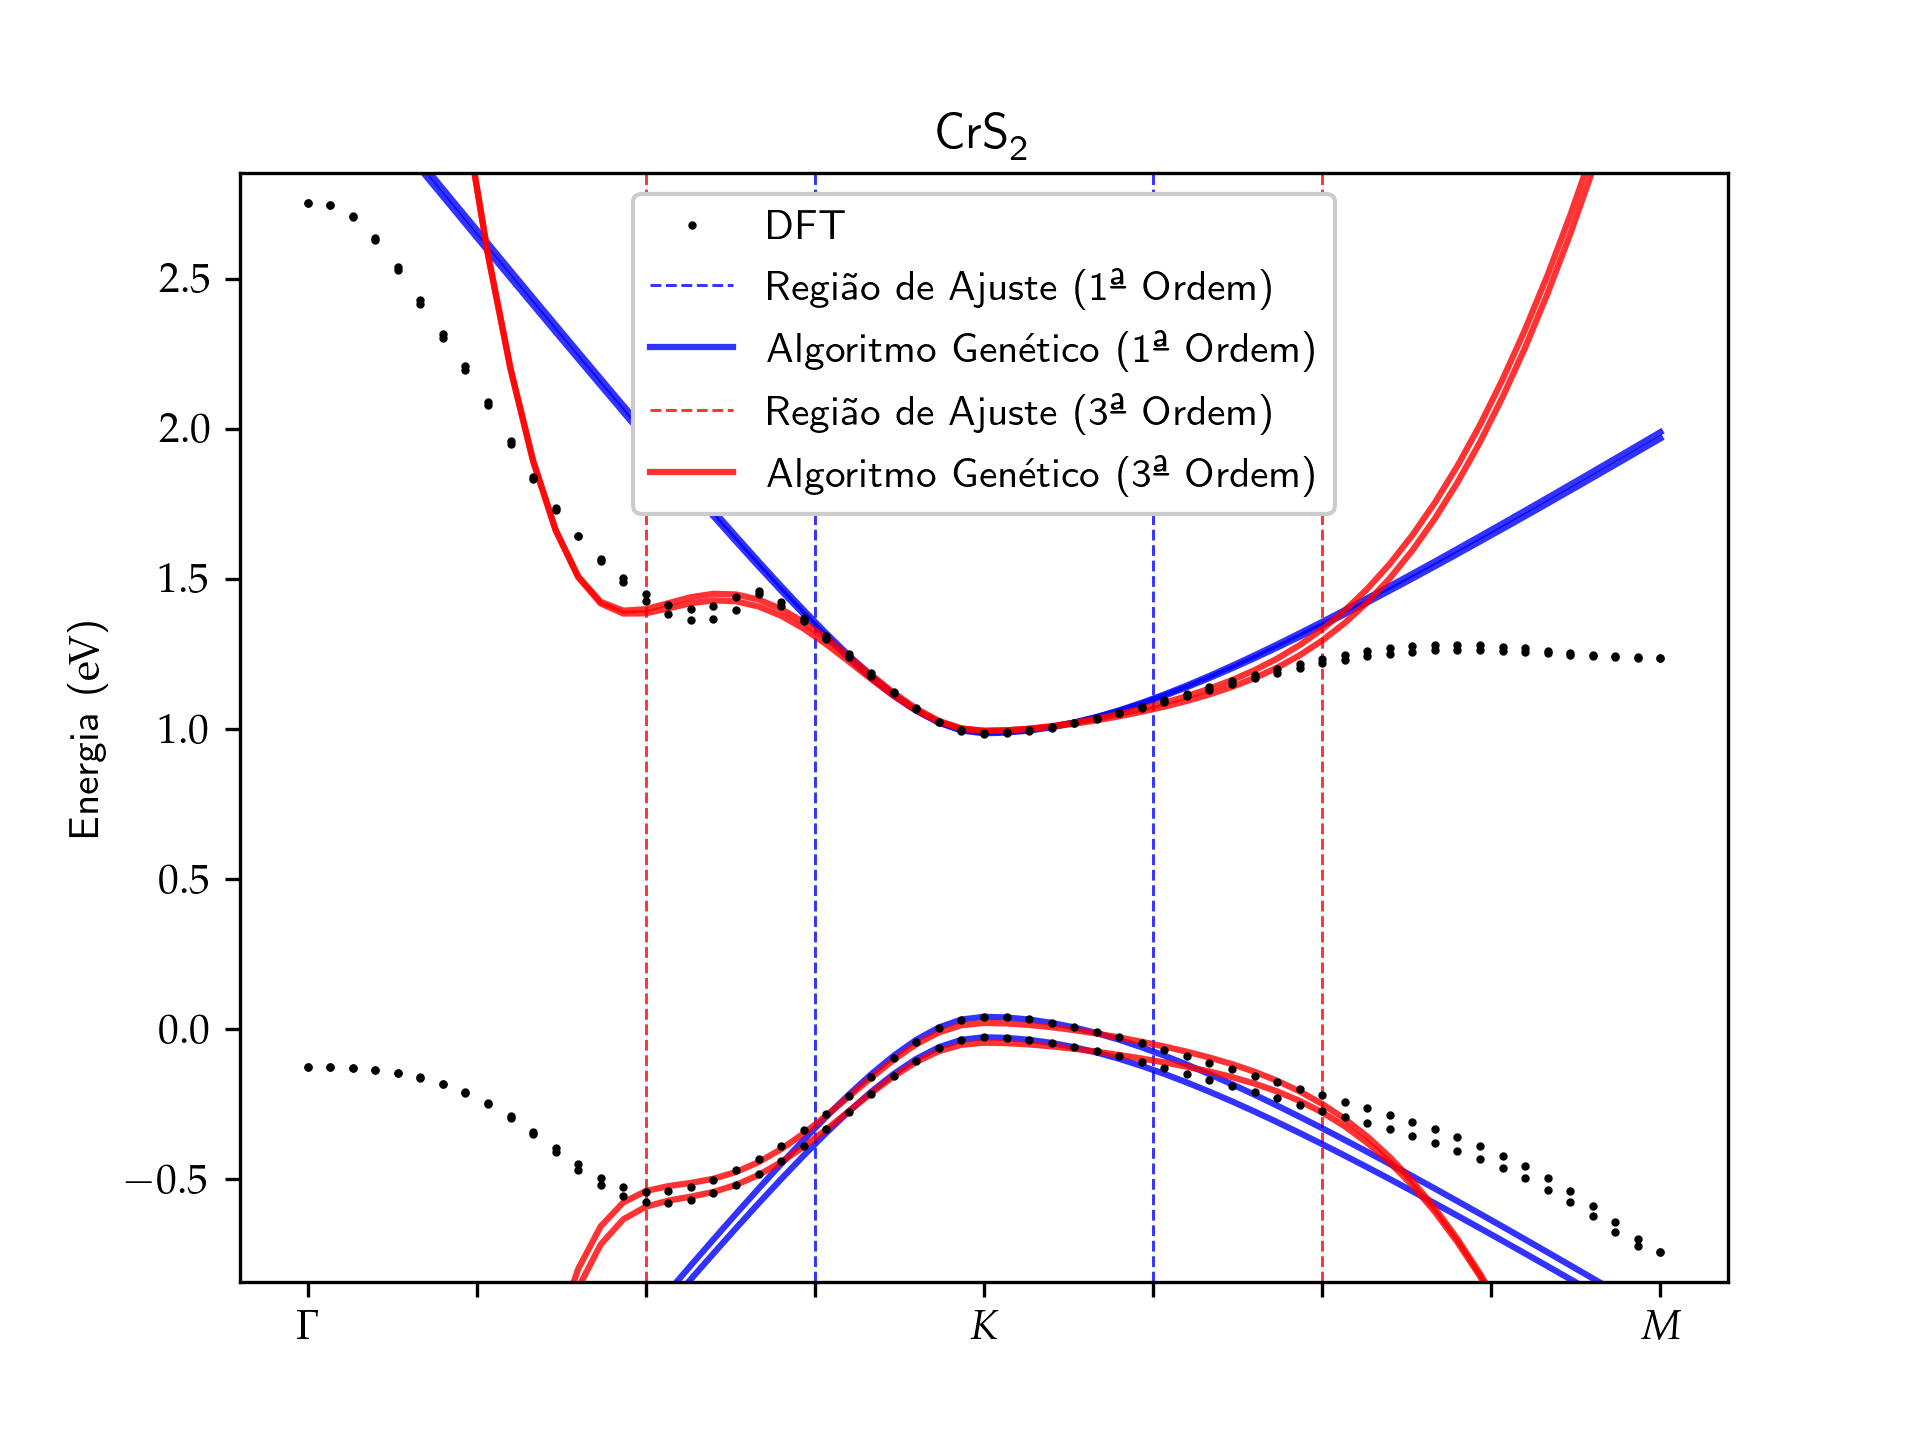
\includegraphics[trim=0 0.6cm 0 0.6cm,clip,width=\textwidth]{imagens/crs2_genetic_algorithm_order_13.png}
    \caption{}
    \label{fig:crs2_genetic_algorithm}
  \end{subfigure}
  \begin{subfigure}{\textwidth}
    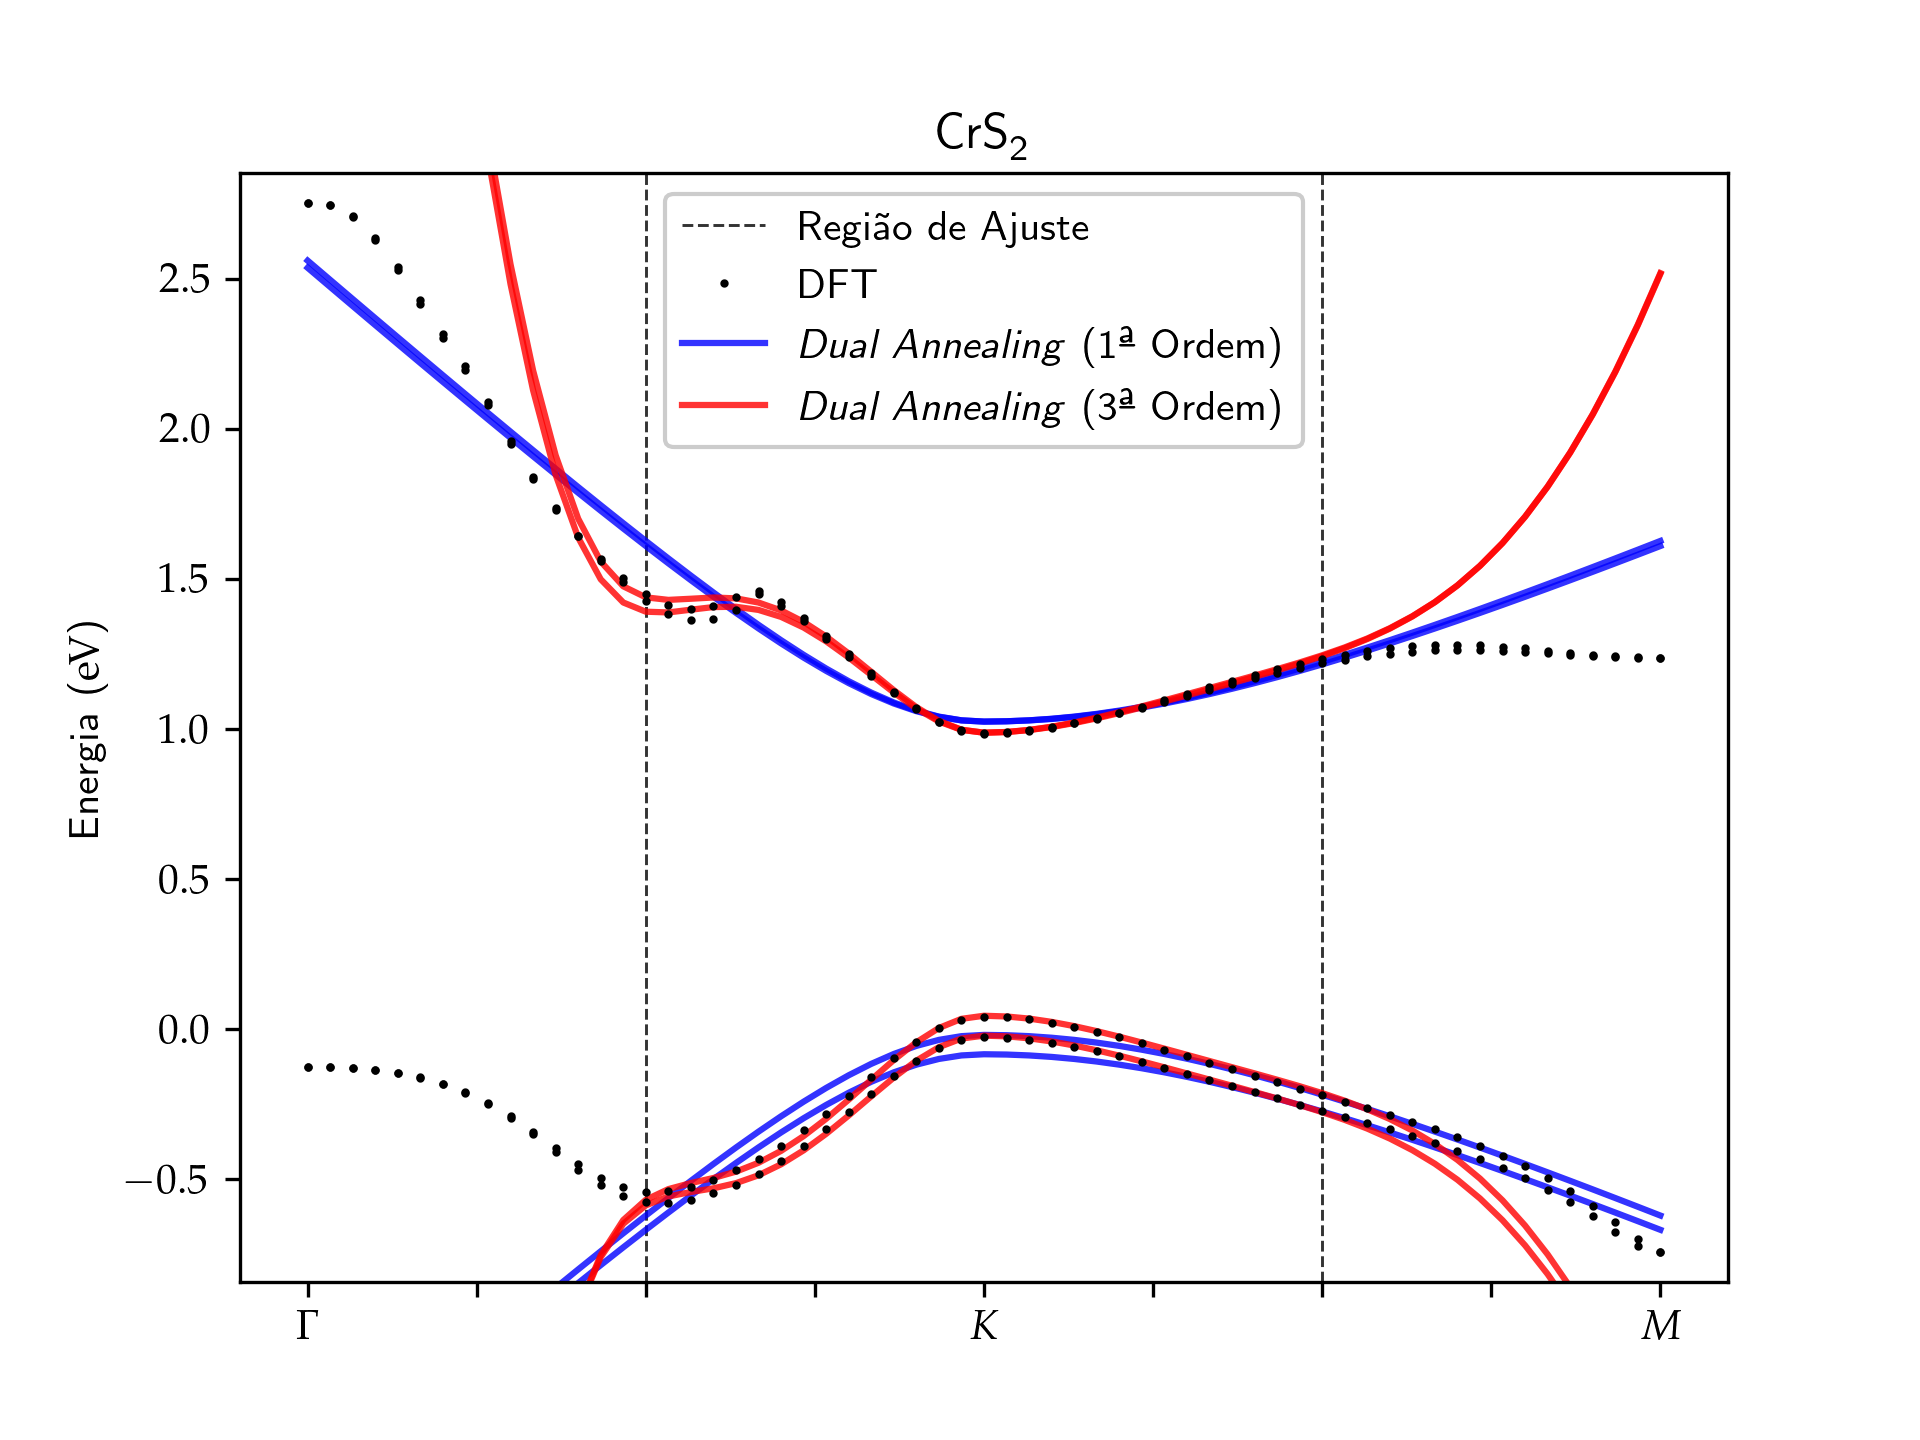
\includegraphics[trim=0 0.6cm 0 0.6cm,clip,width=\textwidth]{imagens/crs2_dual_annealing_order_13.png}
    \caption{}
    \label{fig:crs2_dual_annealing}
  \end{subfigure}
  \caption{
    Gráficos das bandas de energia ajustadas para \ch{CrS2} via Algoritmo Genético
    \subref{fig:crs2_genetic_algorithm} e via \textit{Dual Annealing} \subref{fig:crs2_dual_annealing}
    usando as expansões de 1ª e 3ª ordem de $ \hat{H}_{kp} $.
  }
  \label{fig:crs2}
\end{figure}

\begin{figure}[p]
  \centering
  \begin{subfigure}{\textwidth}
    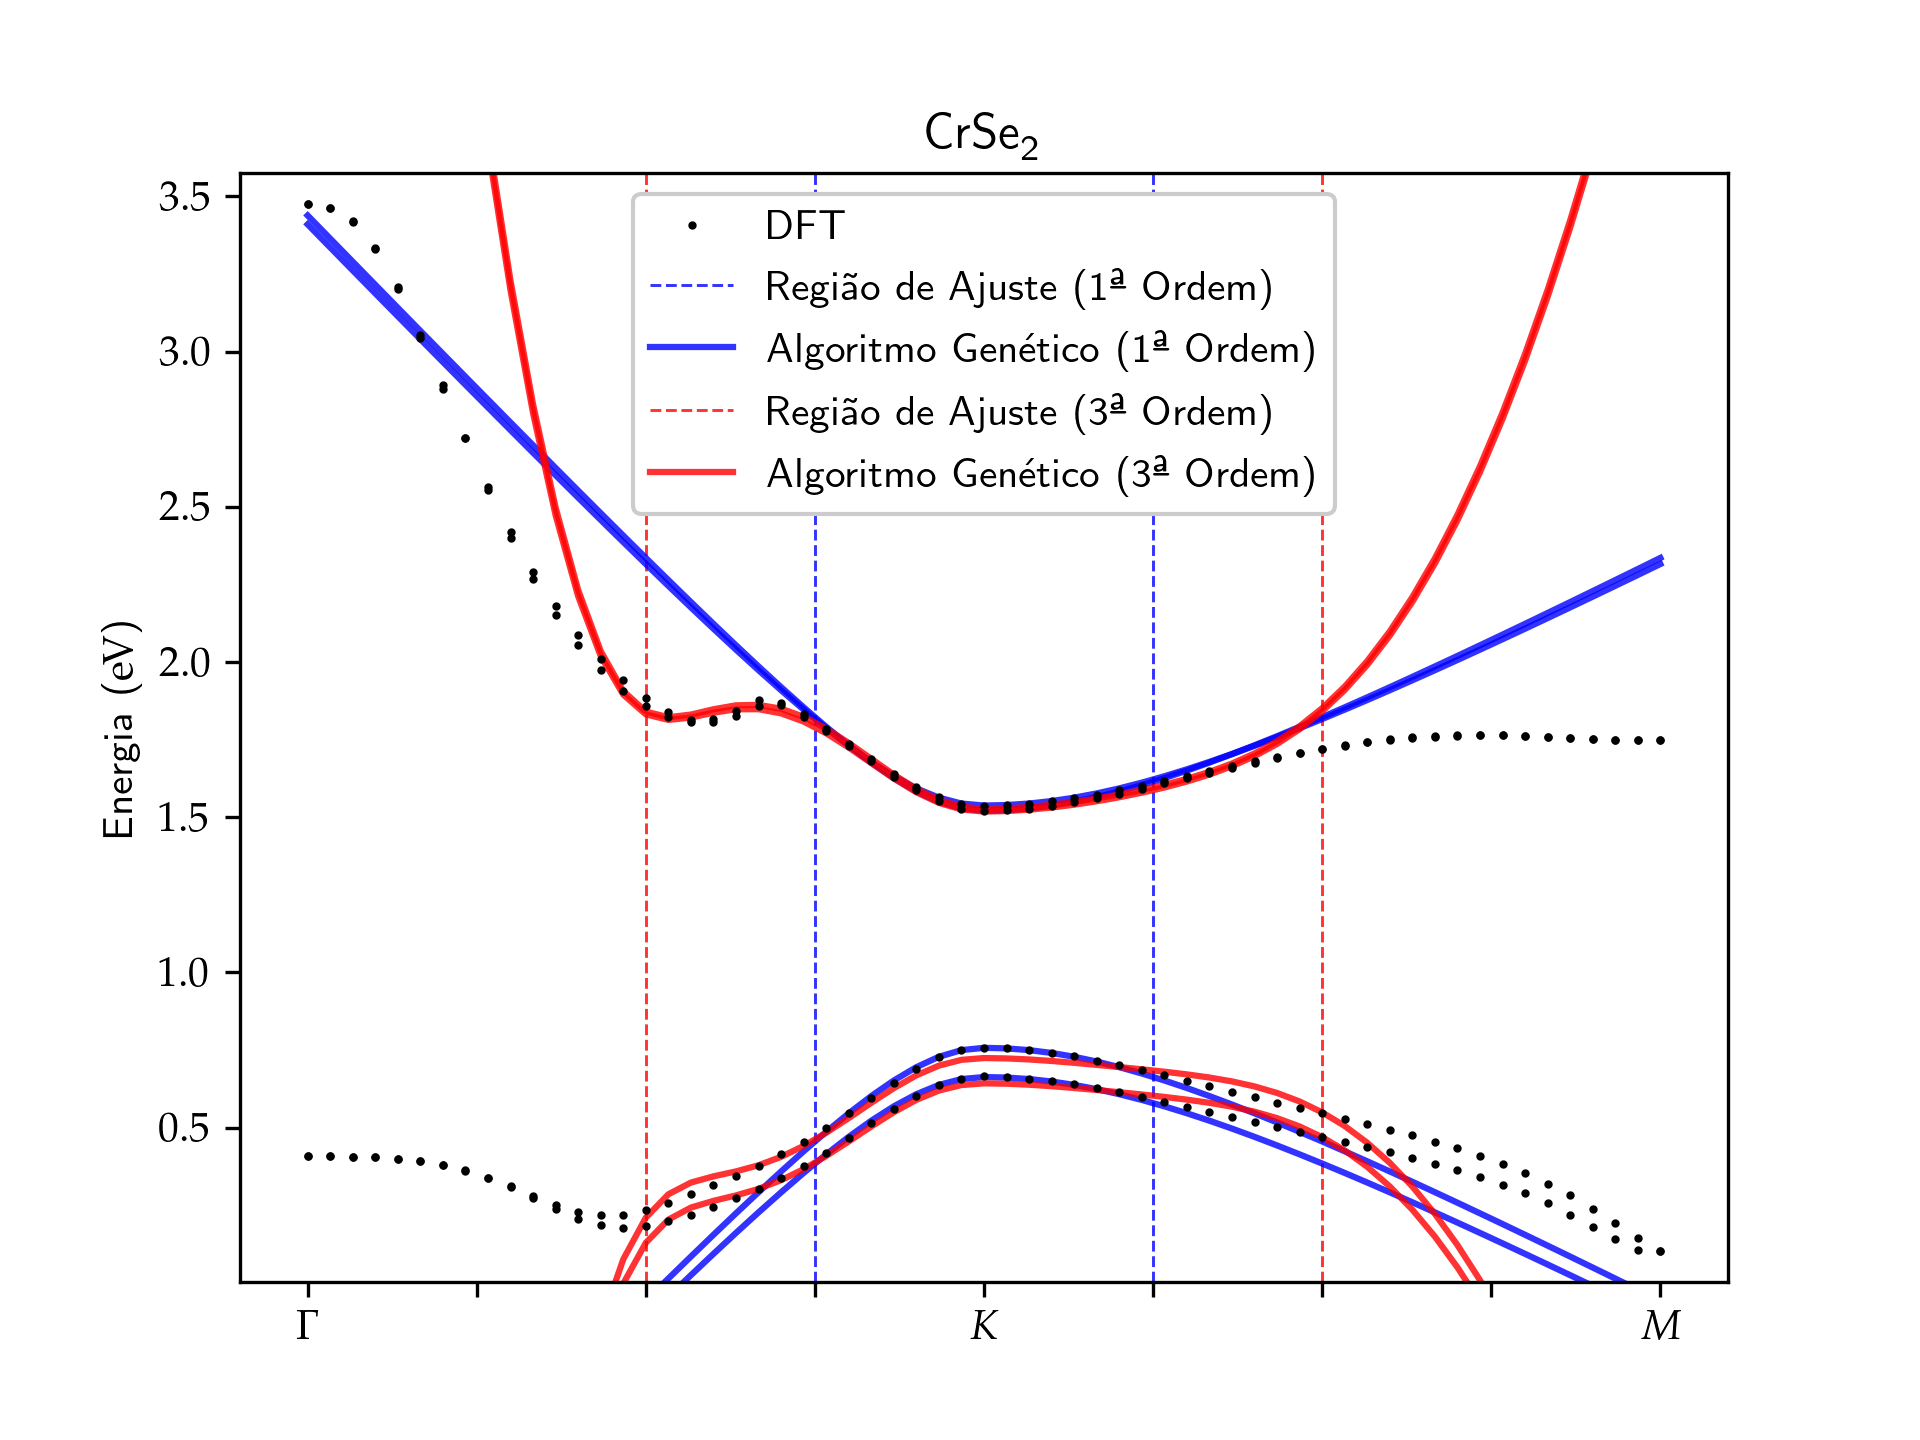
\includegraphics[trim=0 0.6cm 0 0.6cm,clip,width=\textwidth]{imagens/crse2_genetic_algorithm_order_13.png}
    \caption{}
    \label{fig:crse2_genetic_algorithm}
  \end{subfigure}
  \begin{subfigure}{\textwidth}
    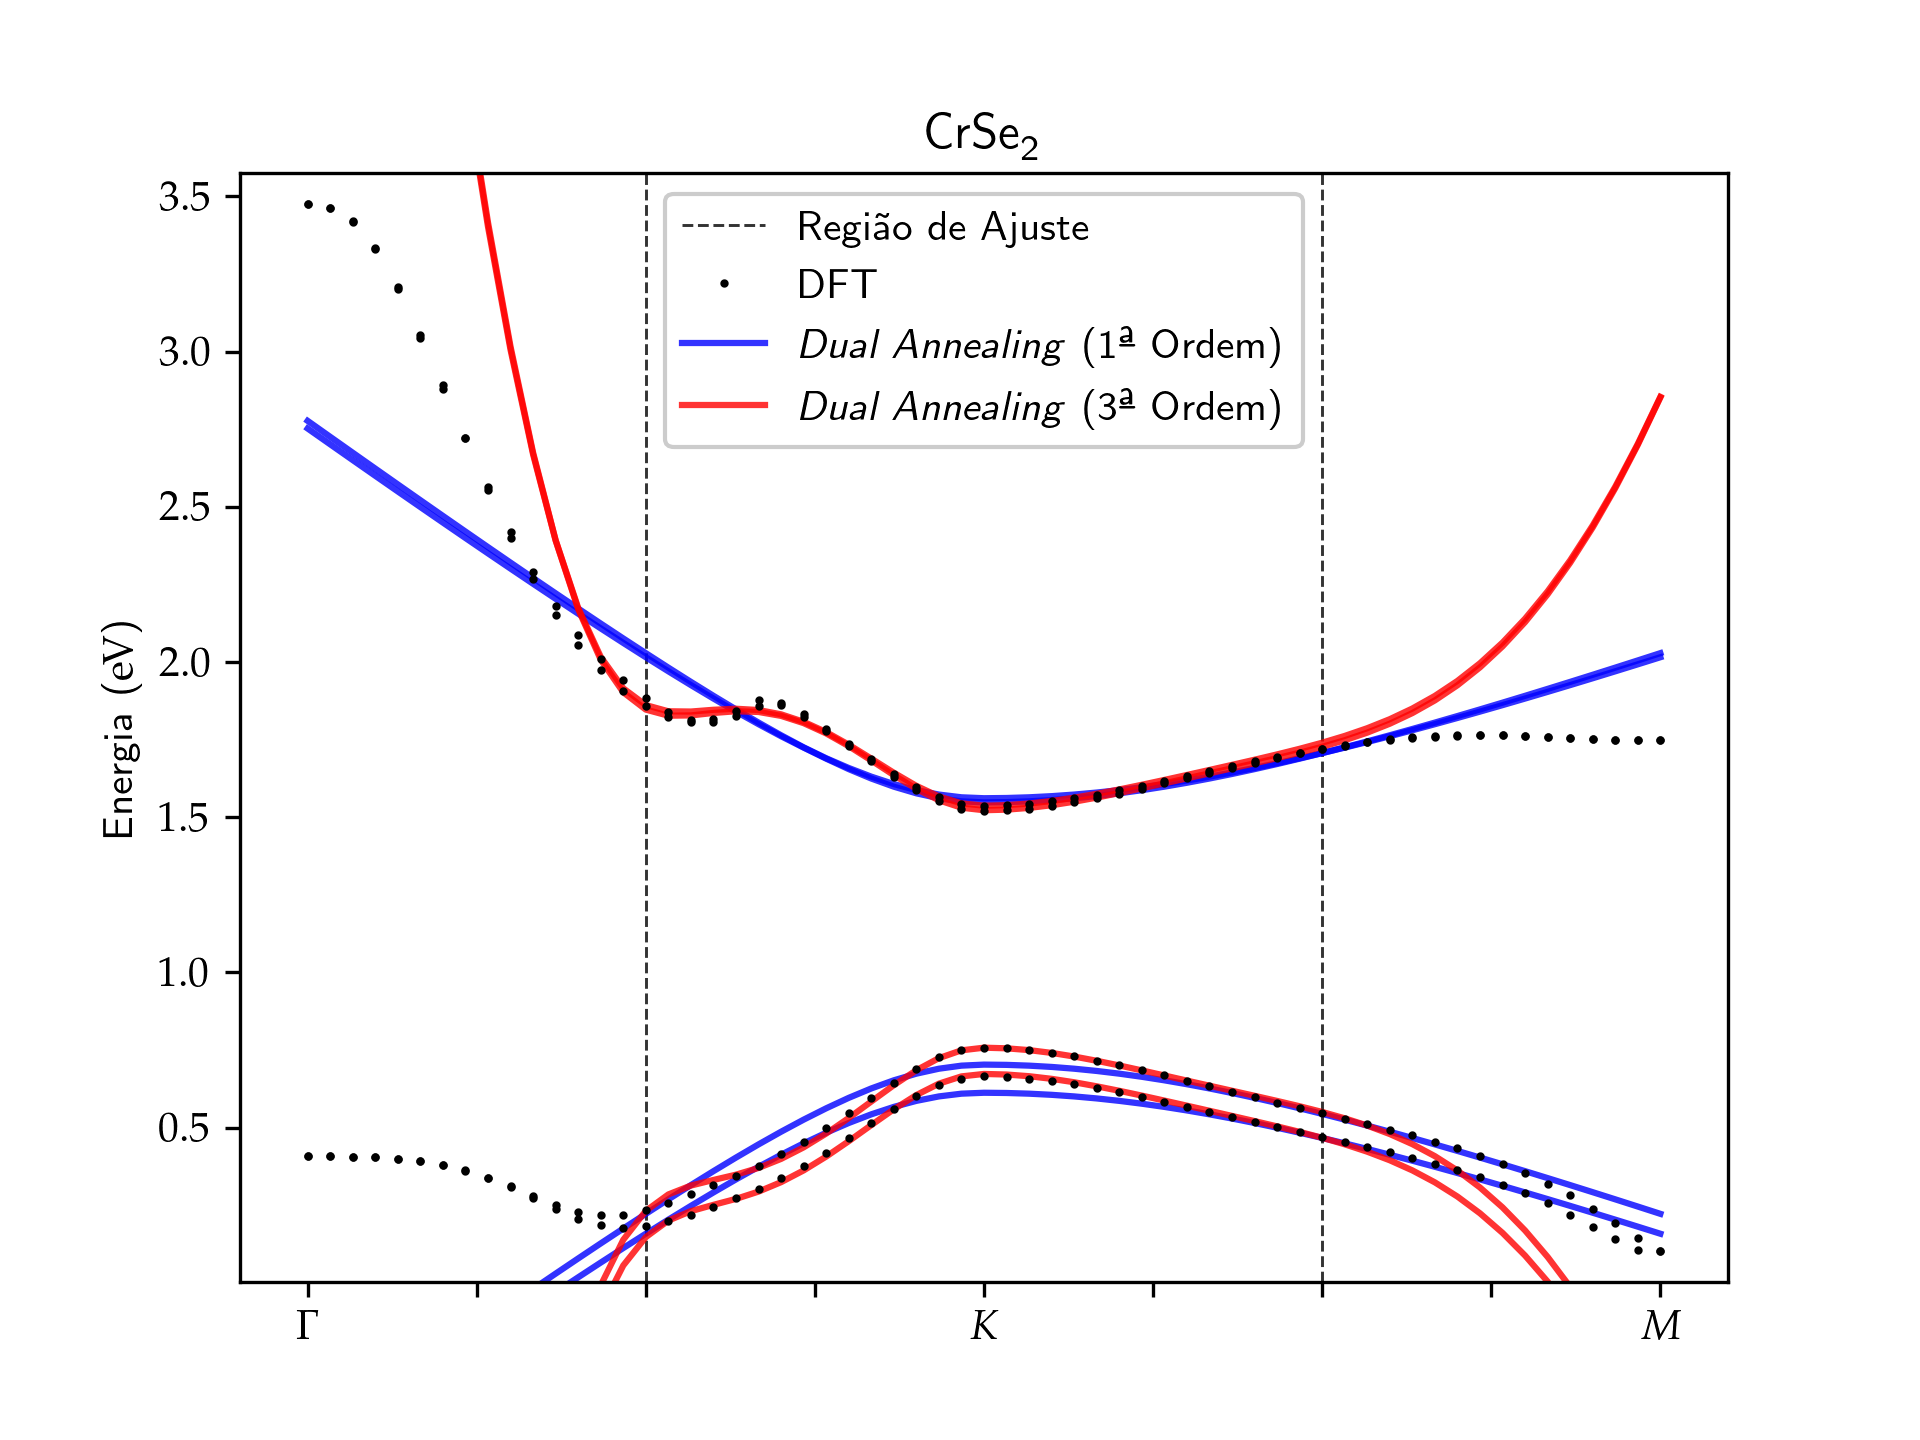
\includegraphics[trim=0 0.6cm 0 0.6cm,clip,width=\textwidth]{imagens/crse2_dual_annealing_order_13.png}
    \caption{}
    \label{fig:crse2_dual_annealing}
  \end{subfigure}
  \caption{
    Gráficos das bandas de energia ajustadas para \ch{CrSe2} via Algoritmo Genético
    \subref{fig:crse2_genetic_algorithm} e via \textit{Dual Annealing}
    \subref{fig:crse2_dual_annealing} usando as expansões de 1ª e 3ª ordem de $ \hat{H}_{kp} $.
  }
  \label{fig:crse2}
\end{figure}

\begin{figure}[p]
  \centering
  \begin{subfigure}{\textwidth}
    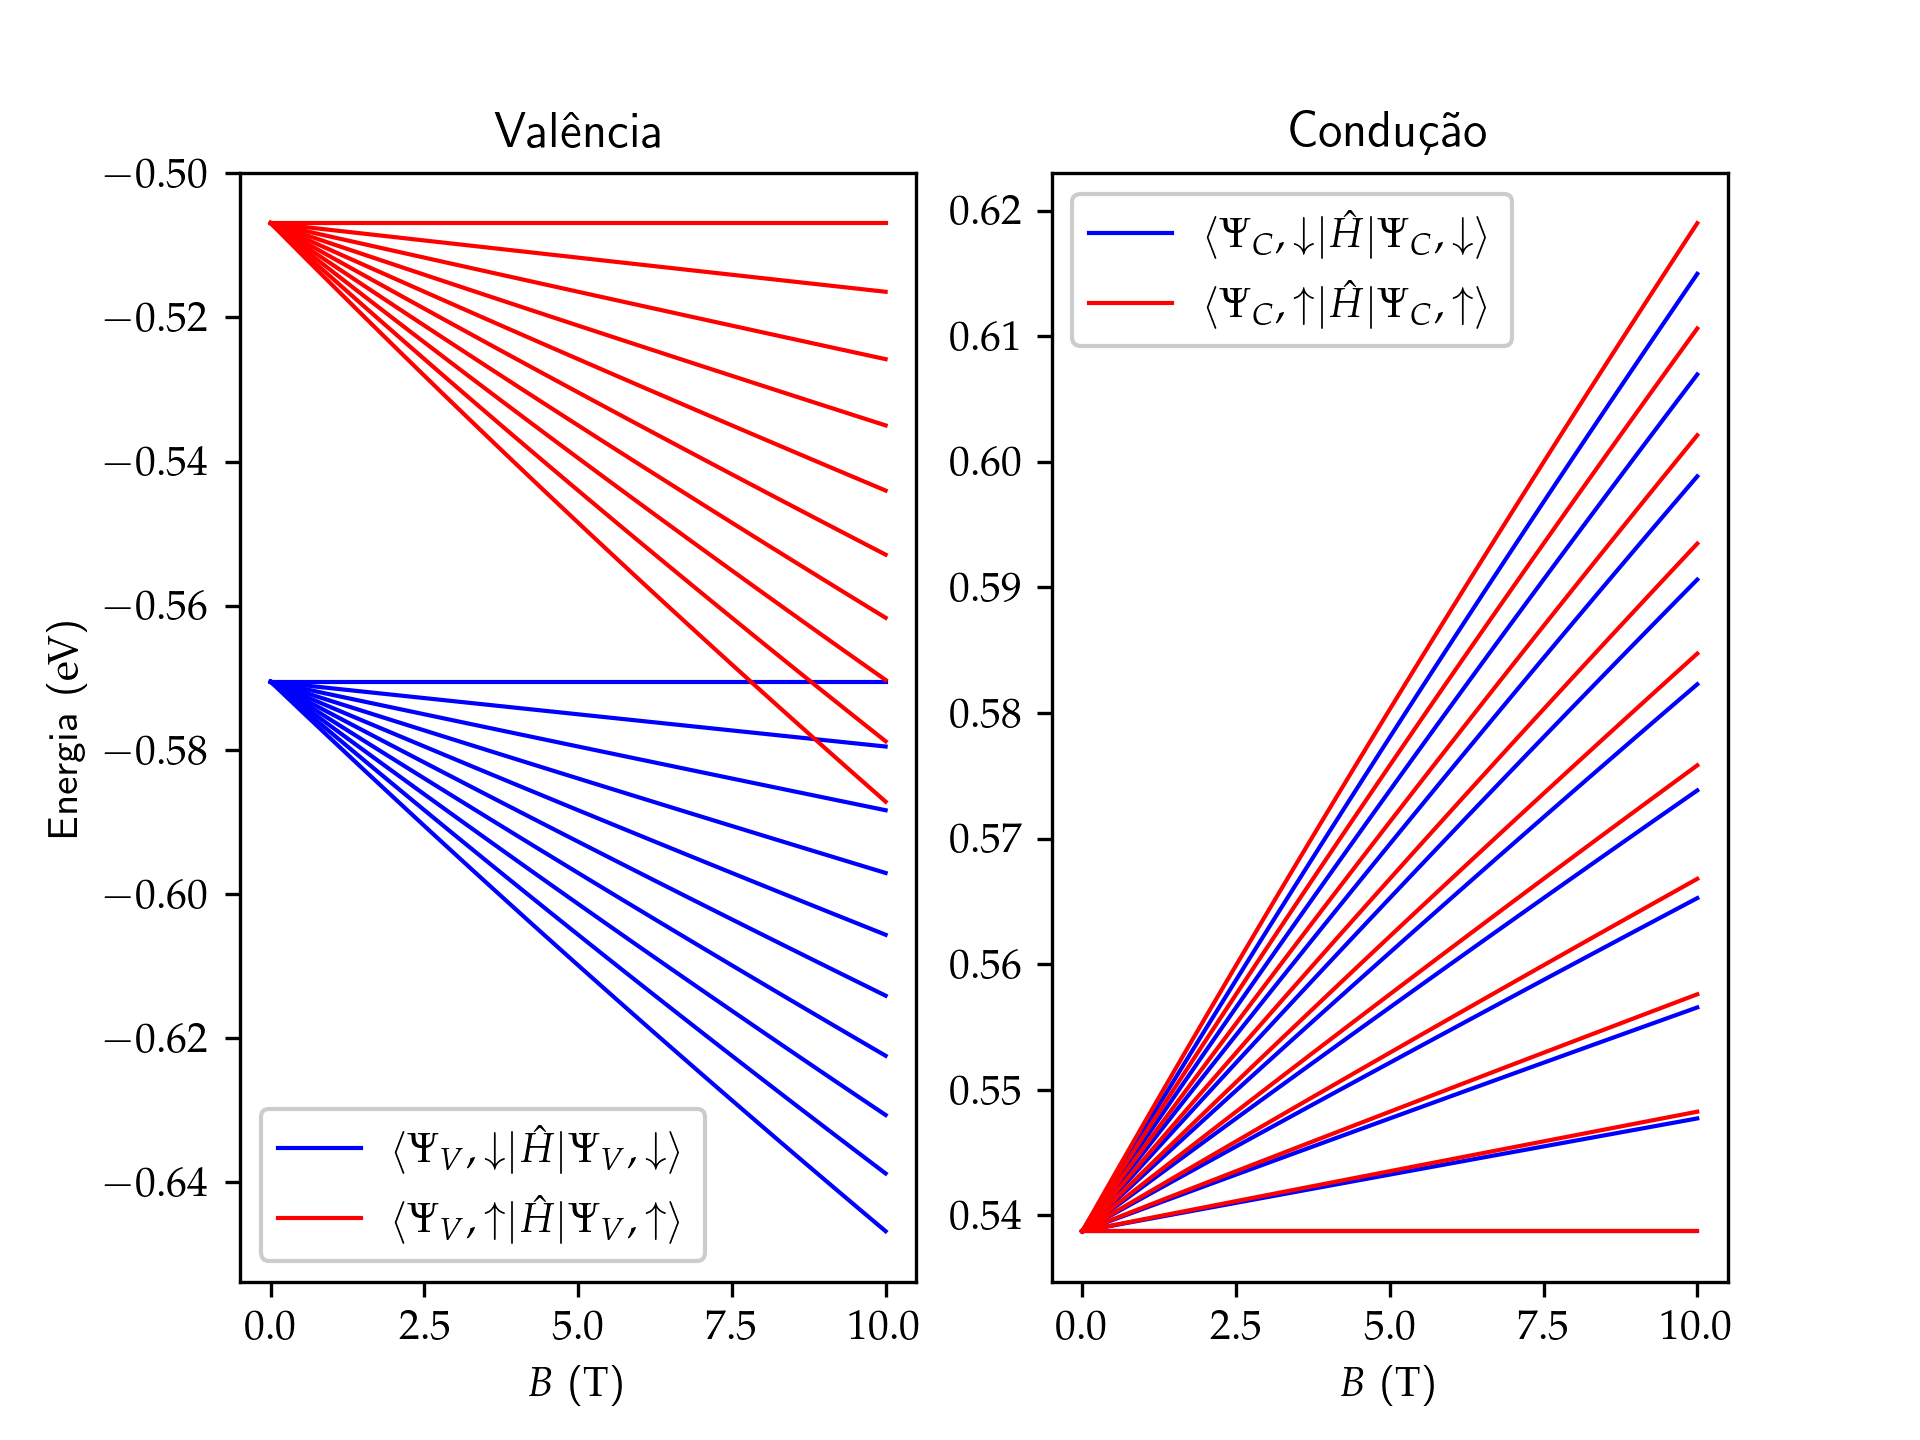
\includegraphics[width=\textwidth]{imagens/crs2_landau_levels.png}
    \caption{}
    \label{fig:crs2_landau_levels}
  \end{subfigure}
  \begin{subfigure}{0.9\textwidth}
    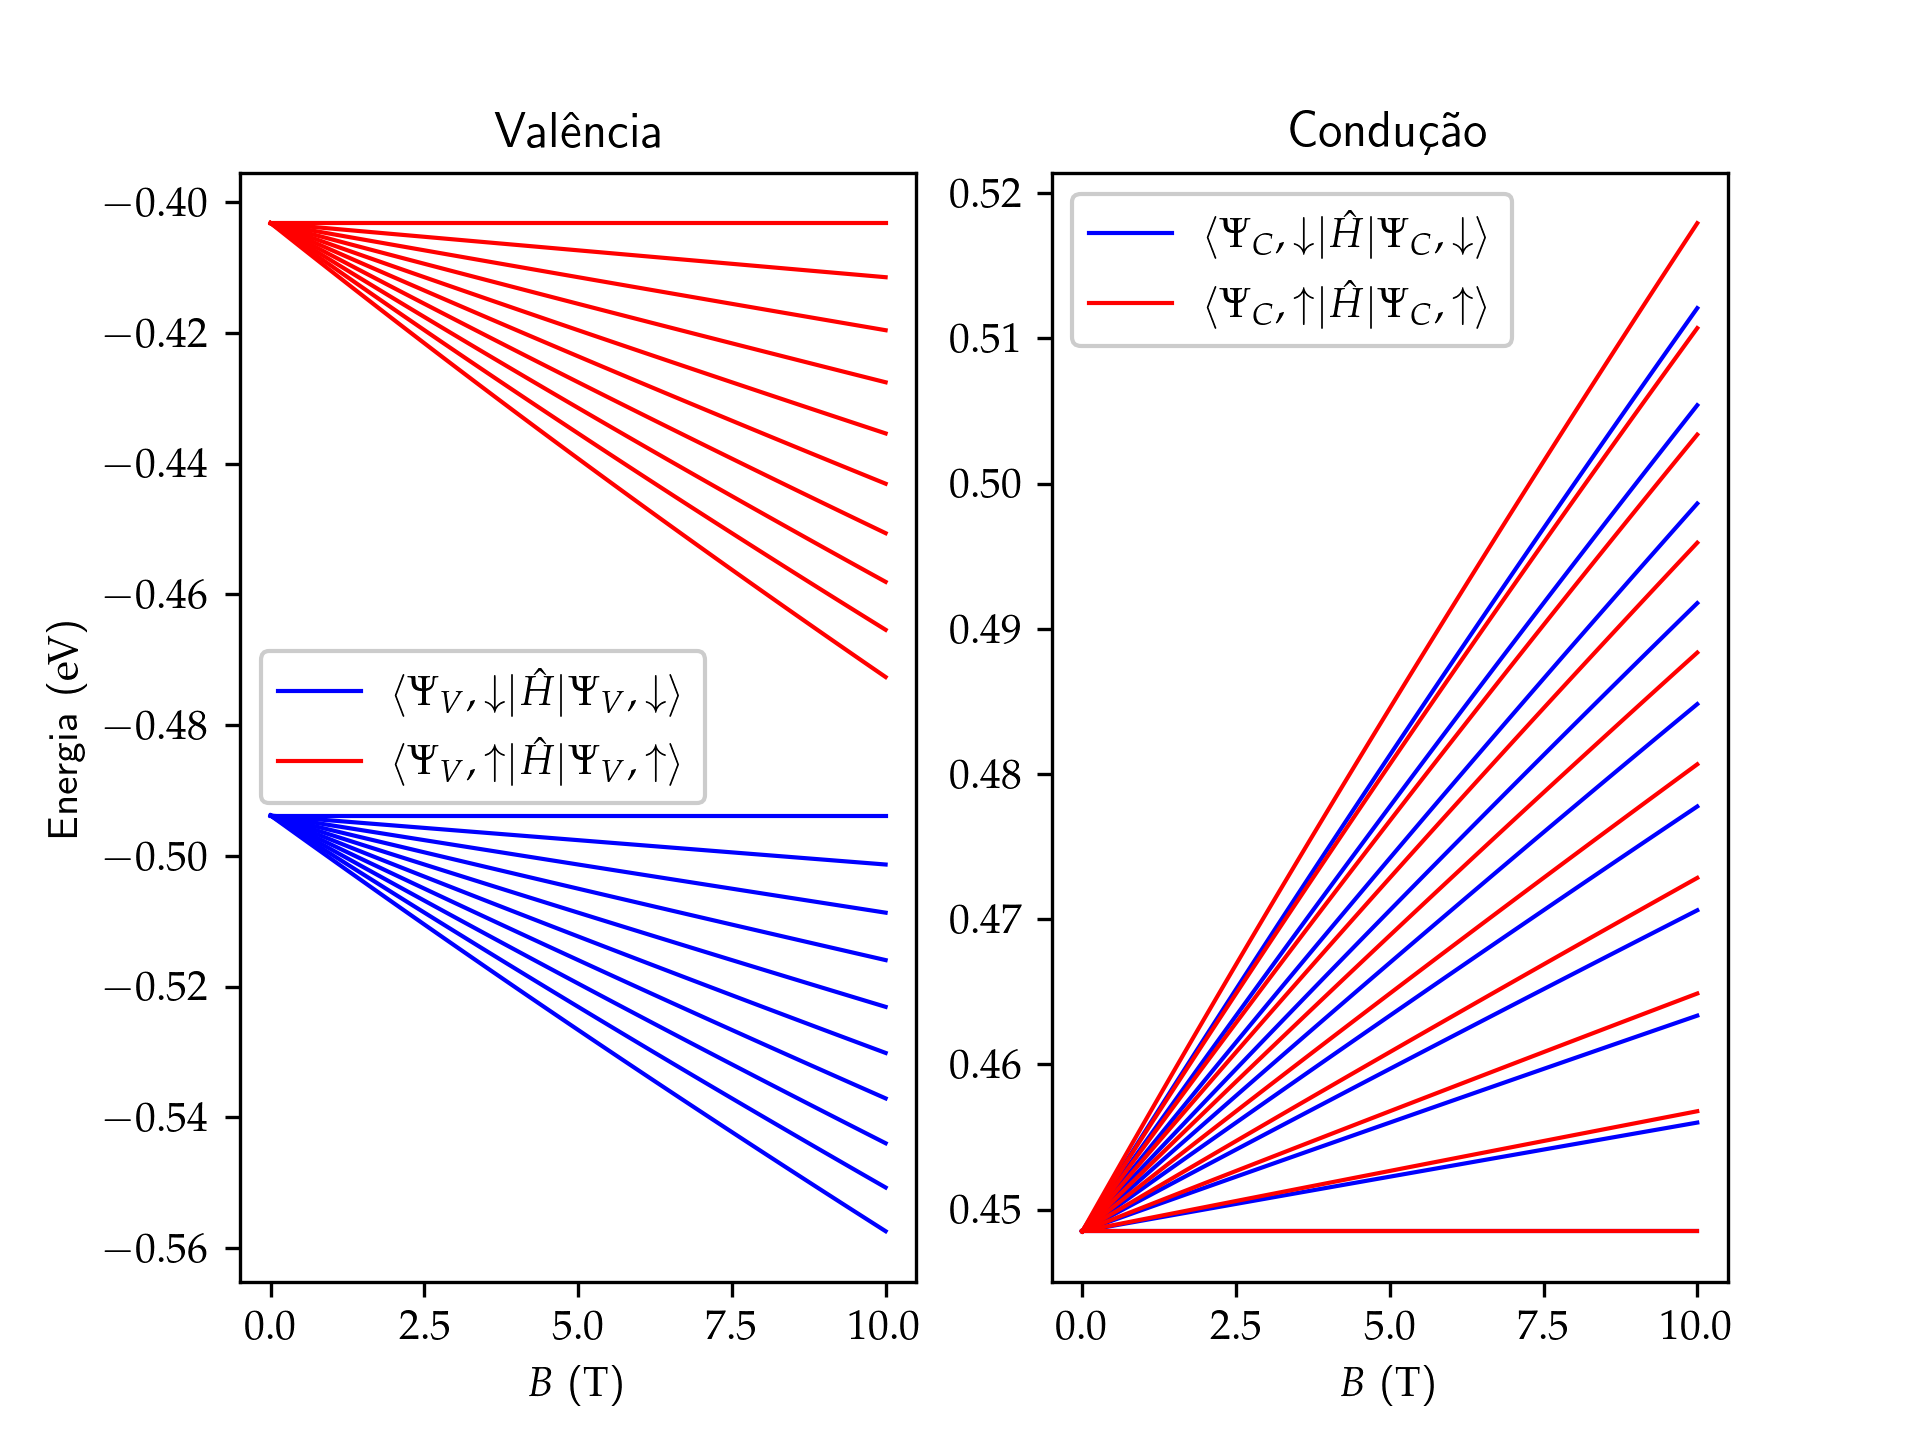
\includegraphics[width=\textwidth]{imagens/crse2_landau_levels.png}
    \caption{}
    \label{fig:crse2_landau_levels}
  \end{subfigure}
  \caption{
    Gráficos dos níveis de Landau para os materiais \ch{CrS2}
    \subref{fig:crs2_landau_levels} e \ch{CrSe2}
    \subref{fig:crse2_landau_levels} em termos do campo magnético externo
    aplicado na direção normal à respectiva monocamada.
  }
  \label{fig:landau_levels}
\end{figure}



\section{Testes de Performance}

Em testes de tempo de execução o programa escalou bem, sendo sua complexidade temporal $\mathcal{O}(n)$ para o
tamanho de população, e $\mathcal{O}(g)$ para número de gerações decorridas. 
Nas figuras exibidas nesse capítulo, o tempo médio decorrido na evolução das populações de 1000 indivíduos
foi de 15 segundos\footnote{
  Tempo obtido usando uma máquina com processador Intel i7-8550U com frequência máxima de 4GHz.
  É importante frisar aqui as evoluções das 8 populações ocorreram em 8 processos em paralelo.
  Assim, é possível que, para uma única população, os tempos de execução sejam ligeiramente menores.
} enquanto que o tamanho da população necessário para que o processo tomasse mais de uma hora foi
superior a $n = 10^5$, para o mesmo número de gerações.

Isso mostra que a implementação é escalável para grandes valores de $n$, o que pode ser desejável em
algumas aplicações. É posto a prova também a performance da biblioteca NumPy, cujas funções e estruturas
de dados implementadas se mostraram altamente otimizadas.